% Options for packages loaded elsewhere
\PassOptionsToPackage{unicode}{hyperref}
\PassOptionsToPackage{hyphens}{url}
\PassOptionsToPackage{dvipsnames,svgnames,x11names}{xcolor}
%
\documentclass[
  letterpaper,
  DIV=11,
  numbers=noendperiod]{scrreprt}

\usepackage{amsmath,amssymb}
\usepackage{iftex}
\ifPDFTeX
  \usepackage[T1]{fontenc}
  \usepackage[utf8]{inputenc}
  \usepackage{textcomp} % provide euro and other symbols
\else % if luatex or xetex
  \usepackage{unicode-math}
  \defaultfontfeatures{Scale=MatchLowercase}
  \defaultfontfeatures[\rmfamily]{Ligatures=TeX,Scale=1}
\fi
\usepackage{lmodern}
\ifPDFTeX\else  
    % xetex/luatex font selection
\fi
% Use upquote if available, for straight quotes in verbatim environments
\IfFileExists{upquote.sty}{\usepackage{upquote}}{}
\IfFileExists{microtype.sty}{% use microtype if available
  \usepackage[]{microtype}
  \UseMicrotypeSet[protrusion]{basicmath} % disable protrusion for tt fonts
}{}
\makeatletter
\@ifundefined{KOMAClassName}{% if non-KOMA class
  \IfFileExists{parskip.sty}{%
    \usepackage{parskip}
  }{% else
    \setlength{\parindent}{0pt}
    \setlength{\parskip}{6pt plus 2pt minus 1pt}}
}{% if KOMA class
  \KOMAoptions{parskip=half}}
\makeatother
\usepackage{xcolor}
\setlength{\emergencystretch}{3em} % prevent overfull lines
\setcounter{secnumdepth}{5}
% Make \paragraph and \subparagraph free-standing
\makeatletter
\ifx\paragraph\undefined\else
  \let\oldparagraph\paragraph
  \renewcommand{\paragraph}{
    \@ifstar
      \xxxParagraphStar
      \xxxParagraphNoStar
  }
  \newcommand{\xxxParagraphStar}[1]{\oldparagraph*{#1}\mbox{}}
  \newcommand{\xxxParagraphNoStar}[1]{\oldparagraph{#1}\mbox{}}
\fi
\ifx\subparagraph\undefined\else
  \let\oldsubparagraph\subparagraph
  \renewcommand{\subparagraph}{
    \@ifstar
      \xxxSubParagraphStar
      \xxxSubParagraphNoStar
  }
  \newcommand{\xxxSubParagraphStar}[1]{\oldsubparagraph*{#1}\mbox{}}
  \newcommand{\xxxSubParagraphNoStar}[1]{\oldsubparagraph{#1}\mbox{}}
\fi
\makeatother


\providecommand{\tightlist}{%
  \setlength{\itemsep}{0pt}\setlength{\parskip}{0pt}}\usepackage{longtable,booktabs,array}
\usepackage{calc} % for calculating minipage widths
% Correct order of tables after \paragraph or \subparagraph
\usepackage{etoolbox}
\makeatletter
\patchcmd\longtable{\par}{\if@noskipsec\mbox{}\fi\par}{}{}
\makeatother
% Allow footnotes in longtable head/foot
\IfFileExists{footnotehyper.sty}{\usepackage{footnotehyper}}{\usepackage{footnote}}
\makesavenoteenv{longtable}
\usepackage{graphicx}
\makeatletter
\newsavebox\pandoc@box
\newcommand*\pandocbounded[1]{% scales image to fit in text height/width
  \sbox\pandoc@box{#1}%
  \Gscale@div\@tempa{\textheight}{\dimexpr\ht\pandoc@box+\dp\pandoc@box\relax}%
  \Gscale@div\@tempb{\linewidth}{\wd\pandoc@box}%
  \ifdim\@tempb\p@<\@tempa\p@\let\@tempa\@tempb\fi% select the smaller of both
  \ifdim\@tempa\p@<\p@\scalebox{\@tempa}{\usebox\pandoc@box}%
  \else\usebox{\pandoc@box}%
  \fi%
}
% Set default figure placement to htbp
\def\fps@figure{htbp}
\makeatother
% definitions for citeproc citations
\NewDocumentCommand\citeproctext{}{}
\NewDocumentCommand\citeproc{mm}{%
  \begingroup\def\citeproctext{#2}\cite{#1}\endgroup}
\makeatletter
 % allow citations to break across lines
 \let\@cite@ofmt\@firstofone
 % avoid brackets around text for \cite:
 \def\@biblabel#1{}
 \def\@cite#1#2{{#1\if@tempswa , #2\fi}}
\makeatother
\newlength{\cslhangindent}
\setlength{\cslhangindent}{1.5em}
\newlength{\csllabelwidth}
\setlength{\csllabelwidth}{3em}
\newenvironment{CSLReferences}[2] % #1 hanging-indent, #2 entry-spacing
 {\begin{list}{}{%
  \setlength{\itemindent}{0pt}
  \setlength{\leftmargin}{0pt}
  \setlength{\parsep}{0pt}
  % turn on hanging indent if param 1 is 1
  \ifodd #1
   \setlength{\leftmargin}{\cslhangindent}
   \setlength{\itemindent}{-1\cslhangindent}
  \fi
  % set entry spacing
  \setlength{\itemsep}{#2\baselineskip}}}
 {\end{list}}
\usepackage{calc}
\newcommand{\CSLBlock}[1]{\hfill\break\parbox[t]{\linewidth}{\strut\ignorespaces#1\strut}}
\newcommand{\CSLLeftMargin}[1]{\parbox[t]{\csllabelwidth}{\strut#1\strut}}
\newcommand{\CSLRightInline}[1]{\parbox[t]{\linewidth - \csllabelwidth}{\strut#1\strut}}
\newcommand{\CSLIndent}[1]{\hspace{\cslhangindent}#1}

\KOMAoption{captions}{tableheading}
\makeatletter
\@ifpackageloaded{bookmark}{}{\usepackage{bookmark}}
\makeatother
\makeatletter
\@ifpackageloaded{caption}{}{\usepackage{caption}}
\AtBeginDocument{%
\ifdefined\contentsname
  \renewcommand*\contentsname{Table of contents}
\else
  \newcommand\contentsname{Table of contents}
\fi
\ifdefined\listfigurename
  \renewcommand*\listfigurename{List of Figures}
\else
  \newcommand\listfigurename{List of Figures}
\fi
\ifdefined\listtablename
  \renewcommand*\listtablename{List of Tables}
\else
  \newcommand\listtablename{List of Tables}
\fi
\ifdefined\figurename
  \renewcommand*\figurename{Figure}
\else
  \newcommand\figurename{Figure}
\fi
\ifdefined\tablename
  \renewcommand*\tablename{Table}
\else
  \newcommand\tablename{Table}
\fi
}
\@ifpackageloaded{float}{}{\usepackage{float}}
\floatstyle{ruled}
\@ifundefined{c@chapter}{\newfloat{codelisting}{h}{lop}}{\newfloat{codelisting}{h}{lop}[chapter]}
\floatname{codelisting}{Listing}
\newcommand*\listoflistings{\listof{codelisting}{List of Listings}}
\makeatother
\makeatletter
\makeatother
\makeatletter
\@ifpackageloaded{caption}{}{\usepackage{caption}}
\@ifpackageloaded{subcaption}{}{\usepackage{subcaption}}
\makeatother

\usepackage{bookmark}

\IfFileExists{xurl.sty}{\usepackage{xurl}}{} % add URL line breaks if available
\urlstyle{same} % disable monospaced font for URLs
\hypersetup{
  pdftitle={jump-start-book, last update 2025-09-05},
  pdfauthor={Steve Simon},
  colorlinks=true,
  linkcolor={blue},
  filecolor={Maroon},
  citecolor={Blue},
  urlcolor={Blue},
  pdfcreator={LaTeX via pandoc}}


\title{jump-start-book, last update 2025-09-05}
\author{Steve Simon}
\date{2023-10-03}

\begin{document}
\maketitle

\renewcommand*\contentsname{Table of contents}
{
\hypersetup{linkcolor=}
\setcounter{tocdepth}{2}
\tableofcontents
}

\bookmarksetup{startatroot}

\chapter*{Preface}\label{preface}
\addcontentsline{toc}{chapter}{Preface}

\markboth{Preface}{Preface}

While this book is in progress, I will use the section of the preface to
track my activity (or lack of activity). When the book is complete, the
first section drops and I revert to a normal preface.

On \textbf{2025-09-05}, I moved text that was wrongly placed in chapter
20 back in the correct chapter (19). I started work on chapter 21, but
there is a lot left to be written. I began organizing my bibliography
better. I now have about 11 thousand words total, with four relatively
complete chapters and now three partially completed chapters.

On \textbf{2025-08-29}, I completed a pretty good draft of chapter 20,
writing a methods section. This adds to three other chapters that we
already in good form (chapters 1, 5, and 11). There is also a very
little bit written for chapters 2 and 3. The total word count is just
around 10 thousand, which is a jump from 7 thousand that the book had
been stuck at for many months.

\textbf{The real preface starts here}

This book was a long time coming. I had just finished a book Statistical
Evidence in Medical Trials in 2006, and had a nice idea for a second
book (this one that you are holding right now). It was more or less
written, spread across a few dozen web pages that I had written over the
past eight years. Surely, it would drop right into my lap.

Well, it was just like the John Lennon lyric in ``Beautiful Boy'' about
how life is what happens while you're making other plans. Actually, that
makes it sound like I had a bunch of unexpected (and maybe tragic)
things happed over the past couple of decades. It is actually simpler
than that. There's a computer term, thrashing, that refers to a
multi-tasking computer that spends more time switching from task to task
than in getting any of the tasks done. That's the verb that best
describes my life. I'm thrashing.

Every year I'd show up at the Joint Statistics Meeting and look for the
Cambridge University Press booth. I'd say hello, usually to Lauren
Cowles, sometimes to another representative. This is the year, I'd tell
them, that I'll get the book written. I know exactly what I need to do.
And every year, I'd write a lot less than I intended to. Too much
thrashing.

I turned a corner (slowly) in 2023 when I converted my thin writings
into a book project in Quarto. I really love Quarto and if you have been
using RMarkdown for a while, you should really switch. It's an easy
transition, and everything is so much more intuitive under Quarto.

\textbf{When I really do complete the book, I will add:}

So I'm finally done. It was a long time coming, but it's here. Read on!

\bookmarksetup{startatroot}

\chapter{Introduction}\label{introduction}

This is a great book. Some of the material here is reproduced from my
\href{http://www.pmean.com/10/SecondBook.html}{original book proposal},
published in 2010-07-23.

Refer to the \href{http://www.pmean.com/10/Contents.html}{tentative
table of contents}, published 2010-07-24.

This book will explain the next three steps that you have to take at any
stage of your research project and it is targeted to beginning
researchers who are often confused about the research process and are
often unsure about what to do next.

When people come into my office asking for advice about Statistics, they
may be at the beginning, the planning phase of the study. Or they may be
getting their data ready for data analysis. Or they may be figuring out
which data analysis they are supposed to be using. Or they may be
thinking about how to write up all the results. The one thing in common
is that they come to see me when they are ``stuck.'' There are a few
exceptions, people who know what they want to do next and they just want
to run their thoughts by me to get my opinion. But most people, if they
knew what they were supposed to be doing, they'd be doing those things.

So what do I advise people to do when they are stuck? I can't lay out
the entire task in front of them, but I can almost always tell them what
the next few steps should be. If they take their first three steps
carefully, the following steps should eventually become obvious.

I am writing this book to reach people who can't visit me in person.
This book is for you if you have to struggle with a research project,
especially your first major research project, and you want guidance on
how to best proceed. The examples I give will be targeted to a medical
research setting and to studies involving humans, but should be broadly
applicable to other research areas, especially research in the social
sciences.

There's a certain amount of arrogance in writing a book and expecting
people to pay good money to read it. I'm certainly arrogant enough, but
I hope this book will justify that arrogance. I do have more than 25
years of consulting experience in academic settings, in the federal
government, in a hospital, and as an independent consultant. The one
advantage of being old is that I've seen it all before. I could not have
written this book twenty or even ten years ago.

There's a second level of arrogance, though, in presupposing that I can
offer advice to you without ever having met you and without knowing
anything about your research project. There are certainly some research
projects where the steps I suggest may not make sense, and I apologize
in advance to anyone who has such a project and does not get any benefit
from this book. I do believe, however, that there is a commonality in
most research. In particular, while the final steps in a data analysis
might be impossible to predict, the initial steps can be largely
predicted, based on my experience. And that's what most people need.
Once they get some momentum back in their research project, they usually
find a way to finish things up.

The general advice behind the steps I am suggesting is that you should
never dive into the deep end of the swimming pool first. There's a
natural tendency to tackle the hardest thing first, but this is a
mistake. Instead, wade in gently at the shallow end. Thus, the first
step for a descriptive data analysis is ``know your count'' which means
to know how many observations are in your data set and how many values
are missing in each of your key variables. This sounds like a trivial
step, but you must do this. If you don't know how much data you have,
then you will be likely to overlook important details later on like how
complex of a statistical model might be supported by your data set.

This is not just advice that I offer to you, but advice I follow myself.
When I help out with a new research problem or a new data set, I can't
jump in the deep end either. I need to get comfortable with things.
Small easy steps will help build my confidence before I tackle the big
things.

This book covers the full range of research. The first few chapters talk
about the steps you need to take in designing your research study. A
good research plan, put in writing, is essential for quality research.
No one asks me about how to collect the data, but once they have it,
they need to know how to enter it into the computer, if it is on paper,
or how to import the data into a software package if it comes from an
electronic source.

Once you have data in a program like SPSS, you may not know what
procedures to use. I have chapters on how to start up a descriptive data
analysis (the foundation of all other data analyses), and how to begin
more complex data analyses like linear regression, logistic regression,
and survival data analysis. I use SPSS in my examples for these chapters
because I think it is an ideal statistical package for beginners,
because it is widely available in many academic and medical centers, and
it is easy to explain. But the general principles apply if you are using
SAS, STATA, or any other statistical package.

Finally, once you have all your data analysis, you need to start writing
up your results. I have chapters on how to write the methods section,
results section, and discussion section of a typical research paper.

I can't talk about purely scientific issues. If you're stuck because you
can't get your flow cytometer to work, you won't find any help here.
There is, of course, substantial overlap between science and statistics,
so I won't shy away from talking about this entirely. Just keep in mind
that my comments regarding science are as an outsider and that I do not
have any special expertise except for what little that has rubbed off on
me from the very intelligent scientists and doctors that I have
collaborated with.

There are book out there that offer a more comprehensive overview of
each of these steps. If you are writing a questionnaire, for example,
Alreck and Settle offer complete and thorough advice on what to do.
There are a wide range of books about how to run SPSS, and Julie Pallant
has an excellent one for beginners. If you are interested in what
statistical tests to use when, then Norman and Streiner have an
entertaining and informative book. If you are writing up results for
publication, then look no further than Lang and Secic, a definitive
guide with examples from the published literature and comprehensive
checklists of all the things you need.

What's different about my book is that I am not trying to be a
comprehensive guide that explains every single step that you might
possibly take. Those guides are important but they are also difficult to
read when your concern is not with every single step of the process but
rather in deciding what you should be doing right now.

Each chapter starts with an introduction and then defines the first
three steps that you should take at this stage. Finally, I list some
special cases that can cause special difficulties (the fly in the
ointment) and which might require a more intense interaction with your
statistical consultant.

I do need to place some important limitations. Otherwise, this book
would be impossibly long. I am going to focus on clincial research:
research that focusses directly on the health care of human patients.
Much of the material in this book will still be relevant if you are
working with animals, either for veterinary care or as a mdoel for
testing before testing in humans. But I don't want to talk about how you
obtain human patients in one paragraph and then switch to how you obtain
animal patients in the next paragraph. Likewise, I am going to bypass
some of the special considerations for in vitro studies.

I also do not have the luxury of discussing studies outside of medicine.
If your research involves education, marketing, or political science,
half of the things I discuss will be relevant, but there will also be
special considerations that I cannot address. I'd love to do so, because
these are all such fun and interesting areas of research. But space is
limited and I should focus on the clinical side because that is where
most of my experience is.

\section{Bibliography}\label{bibliography}

Alreck and Settle

Lang and Secic

Noram and Streiner

Fear is often a paralyzing emotion, and it may be just fear itself that
is causing your difficulties. Research is not easy, but don't fool
yourself into thinking that it is beyond your capabilities. You have to
be a very smart person to be in a position where you are capable of
doing an independent research project, so you are more capable than you
might believe. You can get your research project started, and if it is
stalled, you can get a jumpstart that will help you get moving again.
Just focus on what your next three steps should be.

\bookmarksetup{startatroot}

\chapter{Picking a research topic}\label{picking-a-research-topic}

This chapter is based on an email from Ronan Conroy to a statistics
listserv that was
\href{http://new.pmean.com/steps-in-developing-research-ideas/}{reproduced}
on my website.

For some people, picking a research topic is easy. Your boss will tell
you what to work on. For a few jobs, you have enough independence that
you get to choose, but even in those settings, the nature of the company
that you work for will determine what the best research topics are.

The people who have problems picking a research topics are students.
They have to find something suitable for a thesis or dissertation, but
they have never done any serious research before. Where to start, where
to start?

The others who have problems picking a research topic are people working
in a setting that is primarily clinical. The day-to-day demands keep you
busy enough. Even so, you want to do some research, but there is not a
lot of guidance from above. Where to start, where to start?

\section{Step 1. Describe what bothers
you}\label{step-1.-describe-what-bothers-you}

Over many decades, I have learned that irritation is the germ for many
research ideas. it's like that annoying little grain of sand inside an
oyster that turns into a pearl.

So what irritates you? It is either something that you are currently
doing in your job that makes a difference, but no one else is following
your lead. What is wrong with those people? It's obvious to me how
things should be done.

You are not in a position to impose your will on others, so you have to
persuade them. And half of the people you have to persuade are smarter
than you. The other half thinks they are smarter than you.

What will convince such a stubborn group? Well, remember the famous
quote from W. Edwards Deming, ``In God we trust, all others must bring
data.'' He also said, ``Without data, you are just another person with
an opinion.''

Perhaps the best illustration of the importance of data comes from the
Crimean War. Florence Nightingale, the founder of modern nursing. She
toiled in a military hospital caring for wounded soldiers. The death
rates at this hospital were horrific, and most deaths came not from the
battle wounds, but rather from illnesses caught during recuperation.
Through careful sanitation, better nutrition, and other reforms, she
greatly reduced the number of hospital deaths.

Florence Nightingale wanted to see these changes implemented in other
hospitals, getting attention from the authorities, especially for a
woman, was difficult. She devoted herself to collecting statistics,
seeing those as the key to persuasion. And it worked. Her testimony
before various commisions and politicians led to the codification of
many of her reforms.

So if you are doing something that can change the world, get the world
to change by collecting some data.

The flip side of the irritation coin is when you yourself are doing
something that you know isn't working and you'd like to fix it. Think
about what you might change. But don't just change right away. Develop a
plan.

\bookmarksetup{startatroot}

\chapter{Selecting your research
hypothesis}\label{selecting-your-research-hypothesis}

This chapter is based on
\href{http://www.new.pmean.com/steps-in-developing-research-hypothesis/}{one
of my webpages}.

\section{Step 1. Choose an outcome
measure}\label{step-1.-choose-an-outcome-measure}

Do you know, in a quantitative sense, how bad things are right now? If
not, plan how you are going to measure yourself. In other words, define
an outcome measure. Think about what other aspects of your patient care
might be affected by the change and measure them also.

Then think about how you are going to measure the effects of your
change. This is important. Sometimes you change things for the better,
but sometimes your changes have no impact. It's even possible that your
changes could make things worse instead of better.

\section{Step 2. Define your patient
population}\label{step-2.-define-your-patient-population}

Insert text.

\section{Step 3. Select your control
group}\label{step-3.-select-your-control-group}

Insert text.

\section{The fly in the ointment}\label{the-fly-in-the-ointment}

Insert text.

\bookmarksetup{startatroot}

\chapter{Selecting your research
design}\label{selecting-your-research-design}

This chapter is based on several web pages I have written, which I will
find the time to document here.

\section{Step 1. Decide if you can/should
randomize}\label{step-1.-decide-if-you-canshould-randomize}

Insert text.

\section{Step 2. Consider the advantages/disadvantages of retrospective
versus prospective
research}\label{step-2.-consider-the-advantagesdisadvantages-of-retrospective-versus-prospective-research}

Insert text.

\section{Step 3. Think about the most efficient way to select
subjects}\label{step-3.-think-about-the-most-efficient-way-to-select-subjects}

Insert text.

\section{The fly in the ointment}\label{the-fly-in-the-ointment-1}

Insert text.

\section{Bibliography}\label{bibliography-1}

Steve Simon. So you're thinking about a retrospective chart review.
PMean blog, 2016-05-02. Available in
\href{http://blog.pmean.com/chart-review/}{html format}.

\bookmarksetup{startatroot}

\chapter{Selecting your sample size}\label{selecting-your-sample-size}

This chapter is based on
\href{http://www.new.pmean.com/chapter-sample-size/}{one of my web
pages}.

I got an email last week from a client wanting to start a new research
project looking at relationships between parenting beliefs and childhood
behaviors. The description of the sorts of things to examine was quite
elaborate, and it ended with the question ``how many families would we
need to have any significant differences if they exist?'' Unfortunately,
all the elaborate information provided did not include the information I
would need to answer this question. Justifying a sample size usually
involves three steps.

\section{Step 1: Define your research
hypothesis.}\label{step-1-define-your-research-hypothesis.}

Not all research requires a research hypothesis, but most research does,
and until you define that hypothesis, it is impossible to make any
progress on calculating an appropriate sample size. This particular
email provided a fair amount of detail that could be used to derive a
hypothesis, but no formal hypothesis was directly stated. I like to use
the PICO format described in Evidence-Based Medicine to help people
formulate a good research hypothesis. A research hypothesis will usually
(but not always) have four elements:

P: patient population. This is the group of patients that you want to
examine.

I: intervention. This is what you do to the group of patients that you
think will help them improve

C: comparison group. This is the group of patients without the
intervention that you want to compare to.

O: outcome. This is the variable that will indicate whether or not the
intervention is successful.

Sometimes the intervention is not really something that you think will
help the patients but rather an exposure that the patients have to
endure that may produce some bad results.

A well-formulated hypothesis is important, because it tells the
statistician what type of statistic is likely to be needed to test the
hypothesis.

\subsection{What do you do if you don't have a research
hypothesis?}\label{what-do-you-do-if-you-dont-have-a-research-hypothesis}

In some research studies, the goal is exploratory. You don't have a
formal hypothesis at the start of the study, but rather you are hoping
that the data you collect will generate hypotheses for future studies.
The path to selecting a sample size in these settings is quite
different. Often you want to establish that the confidence intervals for
some of the key descriptive statistics in these studies has a reasonable
amount of precision.

\section{Step 2: Find an estimate of the variability of your outcome
measure.}\label{step-2-find-an-estimate-of-the-variability-of-your-outcome-measure.}

You've already done a literature review haven't you? If so, search
through the papers in your review that used the same outcome measure
that you are proposing in your study (the O in PICO). Ideally, the
outcome measure will be examined in a group of patients that is close to
the types of patients that you are studying (the P in PICO, or possibly
the C in PICO). This is not always easy, and you will sometimes be
forced to use a study where the patients are quite different from your
patients. Don't fret too much about this, but make a good faith effort
to find the most representative population that you can.

Some clients will raise an objection here and say that their research is
unique, so it is impossible to find a comparable paper. It is true that
most research is unique (otherwise it wouldn't be research). But what
these people are worried about is that their intervention (the I in
PICO) is unique. In these situations, the remainder of the hypothesis is
usually quite mundane: the patients, the comparison group, and the
outcome (P, C, and O in PICO) are all well studied. If you find a study
where the P, C, and O match reasonably well, but the I doesn't, then you
are probably going to get a good estimate of variation.

If there are major dissimilarities because this patient population (P)
is very different than any previously studied patient population, or
because the outcome measure (O) is newly developed by the researcher,
then perhaps a pilot study would be needed to establish a reasonable
estimate of variation.

Sometimes you can infer a standard deviation through general principles.
If a variable is constrained to be between 0 and 100, it would be
impossible, for example, for the standard deviation to be five thousand.
There are formulas relating the range of a distribution to the standard
deviation that can serve in a pinch if no other data is available. If
your outcome measure is a proportion, for example, then the variation is
related to the estimated proportion. Similarly, the variation in a count
variable is related to the mean of the counts. Find a paper that
establishes a proportion or average count in a control group similar to
your control group and any competent statistician will be able to get an
estimate of variation. In some situations, the amount of variation in a
proportion or count is larger than would be expected by the statistical
distributions (binomial and Poisson) traditionally associated with these
measures. Still, a calculation based on binomial or Poisson assumptions
is a reasonable starting point for further calculations.

\section{Step 3: define the minimum clinically important
difference.}\label{step-3-define-the-minimum-clinically-important-difference.}

The minimum clinically significant difference is the boundary between a
difference so small that no one would adopt the new intervention on the
basis of such a meager changer and a difference large enough to make a
difference (that is, to convince people to change their behavior and
adopt the new therapy).

Establishing the minimum clinically relevant difference is a tricky
task, but it is something that should be done prior to any research
study. It's not easy but this is something that you have to do for
yourself. The clinically relevant difference is determined by medical
experts and not by statisticians. Hey, I'm still trying to understand
the difference between good and bad cholesterol; I wouldn't even be able
to start thinking about how much of a change in cholesterol is
considered clinically relevant. You might start by asking yourself ``How
much of an improvement would I have to see before I would adopt a new
treatment?'' Also, try talking with some of your colleagues. And look at
the size of improvements for other successful treatments.

For binary outcomes, the choice is not too difficult in theory. Suppose
that an intervention ``costs'' X dollars in the sense that it produces
that much pain, discomfort, and inconvenience, in addition to any direct
monetary costs. Suppose the value of a cure is kX where k is a number
greater than 1. A number less than 1, of course, means that even if you
could cure everyone, the costs outweigh the benefits of the cure.

For k\textgreater1, the minimum clinically significant difference in
proportions is 1/k. So if the cure is 10 times more valuable than the
costs, then you need to show at least a 10\% better cure rate (in
absolute terms) than no treatment or the current standard of treatment.
Otherwise, the cure is worse than the disease.

It helps to visualize this with certain types of alternative medicine.
If your treatment is aromatherapy, there is almost no cost involved, so
even a very slight probability of improvement might be worth it. But
Gerson therapy, which involves, among other things, coffee enemas, is a
different story. An enema is reasonably safe, but is not totally risk
free. And it involves a substantially greater level of inconvenience
than aromatherapy. So you'd only adopt Gerson therapy if it helped a
substantial fraction of patients. Exactly how many depends on the dollar
value that you place on having to endure a coffee enema, a task that I
will leave for someone else to quantify.

If there are side effects associated with the treatment that only occur
in a fraction of the patients receiving the treatment, then the
calculations are a bit trickier, but still possible in theory. It
becomes more tricky still when different people place different monetary
values on the risks and inconveniences of a new therapy.

For continuous variables, the minimum clinically significant difference
could be defined as above. Define a threshold that represents ``better''
versus ``not better'' and then try to shift the entire distribution so
that the fraction ``better'' under the new treatment is at least 1/k.

There have also been efforts to elucidate, through experiments,
interviews, and other approaches, what the average person considers an
important shift to be. For the visual analog scale of pain, for example,
a shift of at least 15 mm is considered the smallest value that is
noticeable to the average patient.

\bookmarksetup{startatroot}

\chapter{Developing your pilot study}\label{developing-your-pilot-study}

This chapter is based on \href{http://blog.pmean.com/pilot-study/}{one
of my web pages}.

\section{Step 1. Visualize the bigger study in the
future}\label{step-1.-visualize-the-bigger-study-in-the-future}

Insert text.

\section{Step 2. Identify planning
gaps}\label{step-2.-identify-planning-gaps}

Insert text.

\section{Step 3. Think about where ``Murphy's Law'' might
strike}\label{step-3.-think-about-where-murphys-law-might-strike}

Insert text.

\section{The fly in the ointment}\label{the-fly-in-the-ointment-2}

Insert text.

\section{Bibliography}\label{bibliography-2}

Steve Simon. IRB review of a pilot study. PMean blog, 2007-03-26.
Available in \href{http://www.new.pmean.com/irb-review-pilot/}{html
format}.

Steve Simon. So you're thinking about a pilot study. PMean blog,
2016-06-16. Available in \href{http://blog.pmean.com/pilot-study/}{html
format}.

Steve Simon. Slapping the word pilot on a failed study. PMean blog,
2019-03-03. Available in {[}html format{]}{[}simon-2019{]}.

Steve Simon. The best reasons to run a pilot study. PMean blog,
2023-12-06. Available in
\href{http://new.pmean.com/reasons-to-run-a-pilot/}{html format}.

\bookmarksetup{startatroot}

\chapter{Designing your
questionnaire}\label{designing-your-questionnaire}

This chapter is based on several web pages, that I will add later.

\section{Step 1. Brainstorm a long list and then prune
back}\label{step-1.-brainstorm-a-long-list-and-then-prune-back}

Insert text.

\section{Step 2. Get opinions from content
experts}\label{step-2.-get-opinions-from-content-experts}

Insert text.

\section{Step 3. Pilot test your
questionnaire}\label{step-3.-pilot-test-your-questionnaire}

Insert text.

\section{The fly in the ointment}\label{the-fly-in-the-ointment-3}

Insert text.

\bookmarksetup{startatroot}

\chapter{Obtaining ethical approval for your
study}\label{obtaining-ethical-approval-for-your-study}

This chapter is based on \textless{}\textgreater. Also refer to
\href{http://www.pmean.com/10/Contents.html}{Tentative table of
contents}.

\section{Step 1. Establish your credentials as a
researcher}\label{step-1.-establish-your-credentials-as-a-researcher}

Insert text.

\section{Step 2. Demonstrate your concern for privacy
rights}\label{step-2.-demonstrate-your-concern-for-privacy-rights}

Insert text.

\section{Step 3. Prepare a defensible strategy for your data
analysis}\label{step-3.-prepare-a-defensible-strategy-for-your-data-analysis}

Insert text.

\section{The fly in the ointment}\label{the-fly-in-the-ointment-4}

Insert text.

\bookmarksetup{startatroot}

\chapter{Setting up your data entry
process}\label{setting-up-your-data-entry-process}

This chapter is based on
\href{http://www.pmean.com/99/entry.html}{General guide to data entry}
published 1999-09-03. Also refer to
\href{http://www.pmean.com/10/Contents.html}{Tentative table of
contents}.

\section{Step 1: Arrange your data in a rectangular
format}\label{step-1-arrange-your-data-in-a-rectangular-format}

Add text.

\section{Step 2: Create codes for categorical
data}\label{step-2-create-codes-for-categorical-data}

Add text.

\section{Step 3: Document missing
values}\label{step-3-document-missing-values}

Add text.

\section{The fly in the ointment: longitudinal and repeated measures
data}\label{the-fly-in-the-ointment-longitudinal-and-repeated-measures-data}

Add text.

\bookmarksetup{startatroot}

\chapter{Running a descriptive data
analysis}\label{running-a-descriptive-data-analysis}

This chapter is based on
\href{http://new.pmean.com/steps-in-descriptive-model/}{Steps in a
descriptive model} published 2001-10-11. Also refer to
\href{http://www.pmean.com/10/Contents.html}{Tentative table of
contents}.

\section{Step 1: Know your count}\label{step-1-know-your-count}

Add text.

\section{Step 2: Compute ranges and
frequencies}\label{step-2-compute-ranges-and-frequencies}

Add text.

\section{Step 3: Examine relationships using crosstabs, boxplots, and/or
scatterplots}\label{step-3-examine-relationships-using-crosstabs-boxplots-andor-scatterplots}

Add text.

\section{The fly in the ointment: ordinal
data}\label{the-fly-in-the-ointment-ordinal-data}

Add text.

\bookmarksetup{startatroot}

\chapter{Running a linear regression
analysis}\label{running-a-linear-regression-analysis}

There are two quotes worth mentioning here.

Let no man ignorant of geometry enter - Sign over Plato's Academy in
Athens

Peggy Sue: Well, Mr Snelgrove, I happen to know that in the future I
will not have the slightest use for algebra, and I speak from
experience.

In my talks, I often ask the question, did you like High School Algebra.
I get a mix of responses: some people loved it, some hated it, but most
were indifferent. Fair enough, but if you want to run a linear
regression analysis, you can't be indifferent. If nothing else, you have
to remember the formula you learned in algebra for a straight line.

\(y = mx + b\)

The slope, m, represents the change in y divided by the change in x. The
intercept, b, represents where the line crosses the y-axis.

The linear regression formula is a bit different.

\(\hat{y}_i=\hat\beta_0+\hat\beta_1 X_i\)

where the slope, \(\hat\beta_1\) represents the estimated average change
in Y when X increases by one unit and the intercept, \(\hat\beta_0\),
represents the estimated average value of Y when X equals zero.

\section{Step 1: Plot your data}\label{step-1-plot-your-data}

I've always loved linear regression because it is so visual. You learn a
lot before you compute any statistics by looking at graphs.

\pandocbounded{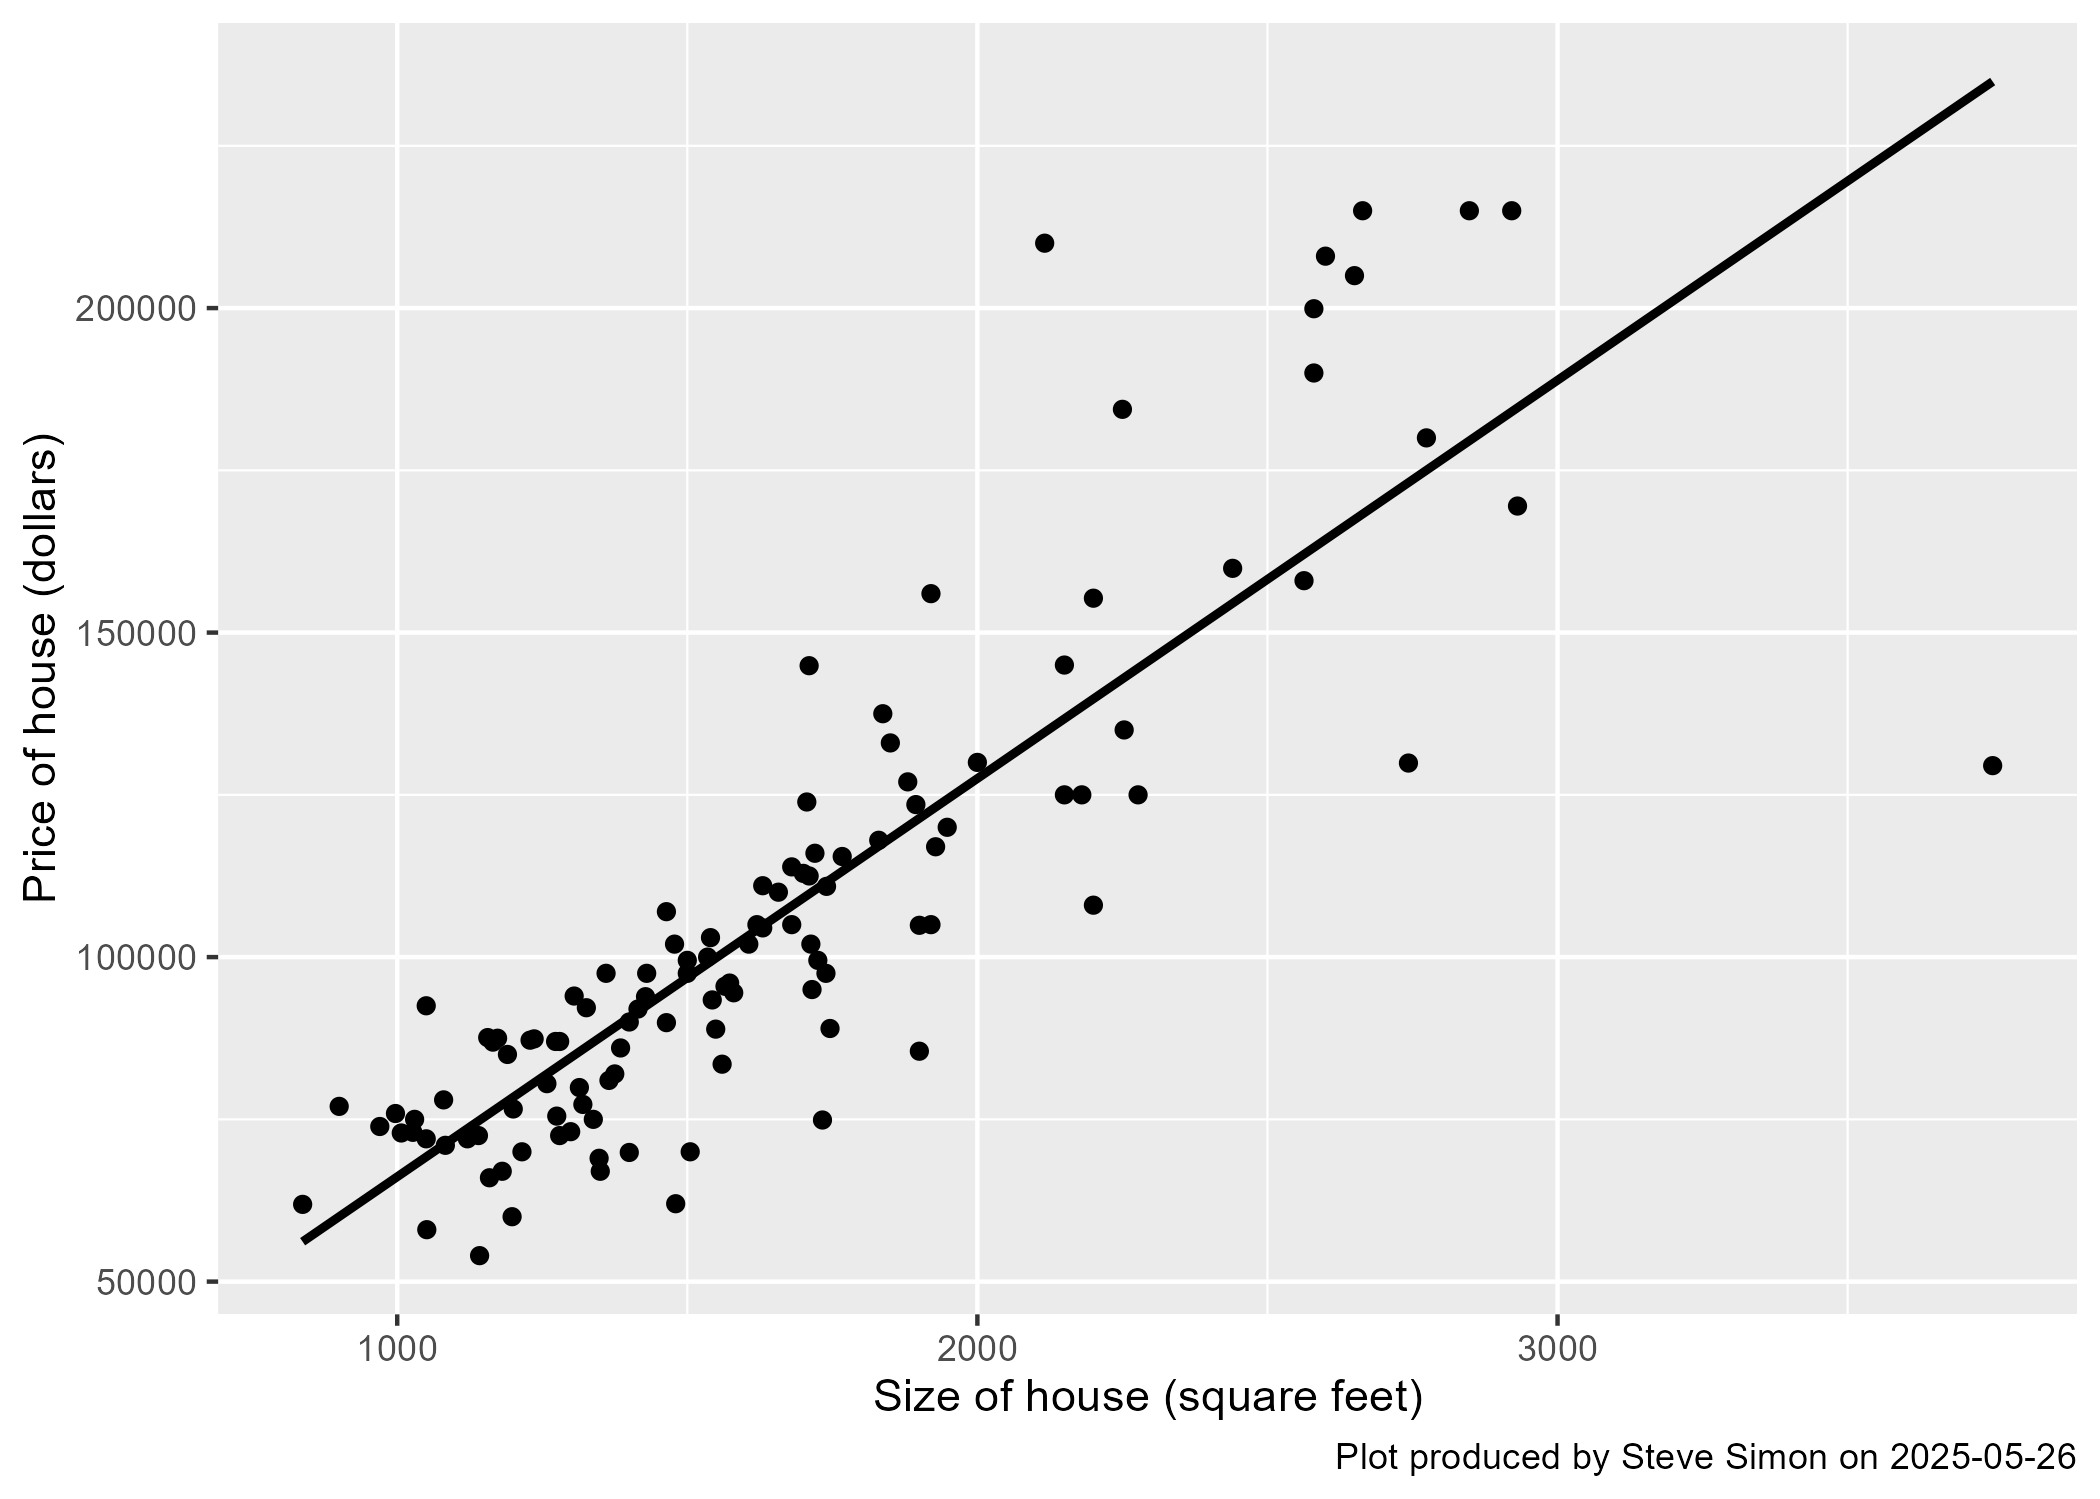
\includegraphics[keepaspectratio]{chapters/../images/figure-11-01.png}}

I added the trend line. You should try to eyeball the slope and
intercept from your graph. You want to see if these values pass the
``smell test.'' Do they seem reasonable or is something a bit fishy and
warrants further investigation.

Here is how you calculate the slope. A thousand square foot house is
predicted to sell for about 70 thousand dollars. A three thousand square
foot house is predicted to sell for about 190 thousand dollars. These
are just rough estimates. Don't worry if you don't get them quite right.

The slope is the change in Y (120 thousand dollars) divided by the
change in X (2 thousand square feet), which produces a rough estimate of
your slope, 60 dollars per square foot. That passes the smell test. It
seems eminently reasonable, especially considering that these are 1993
houses.

To calculate the intercept, you need to redraw the graph so that you can
read the prediction at x=0. Here's what that graph looks like. I
extended the line beyond the range of the data, which is a something
that you should do with great caution.

\pandocbounded{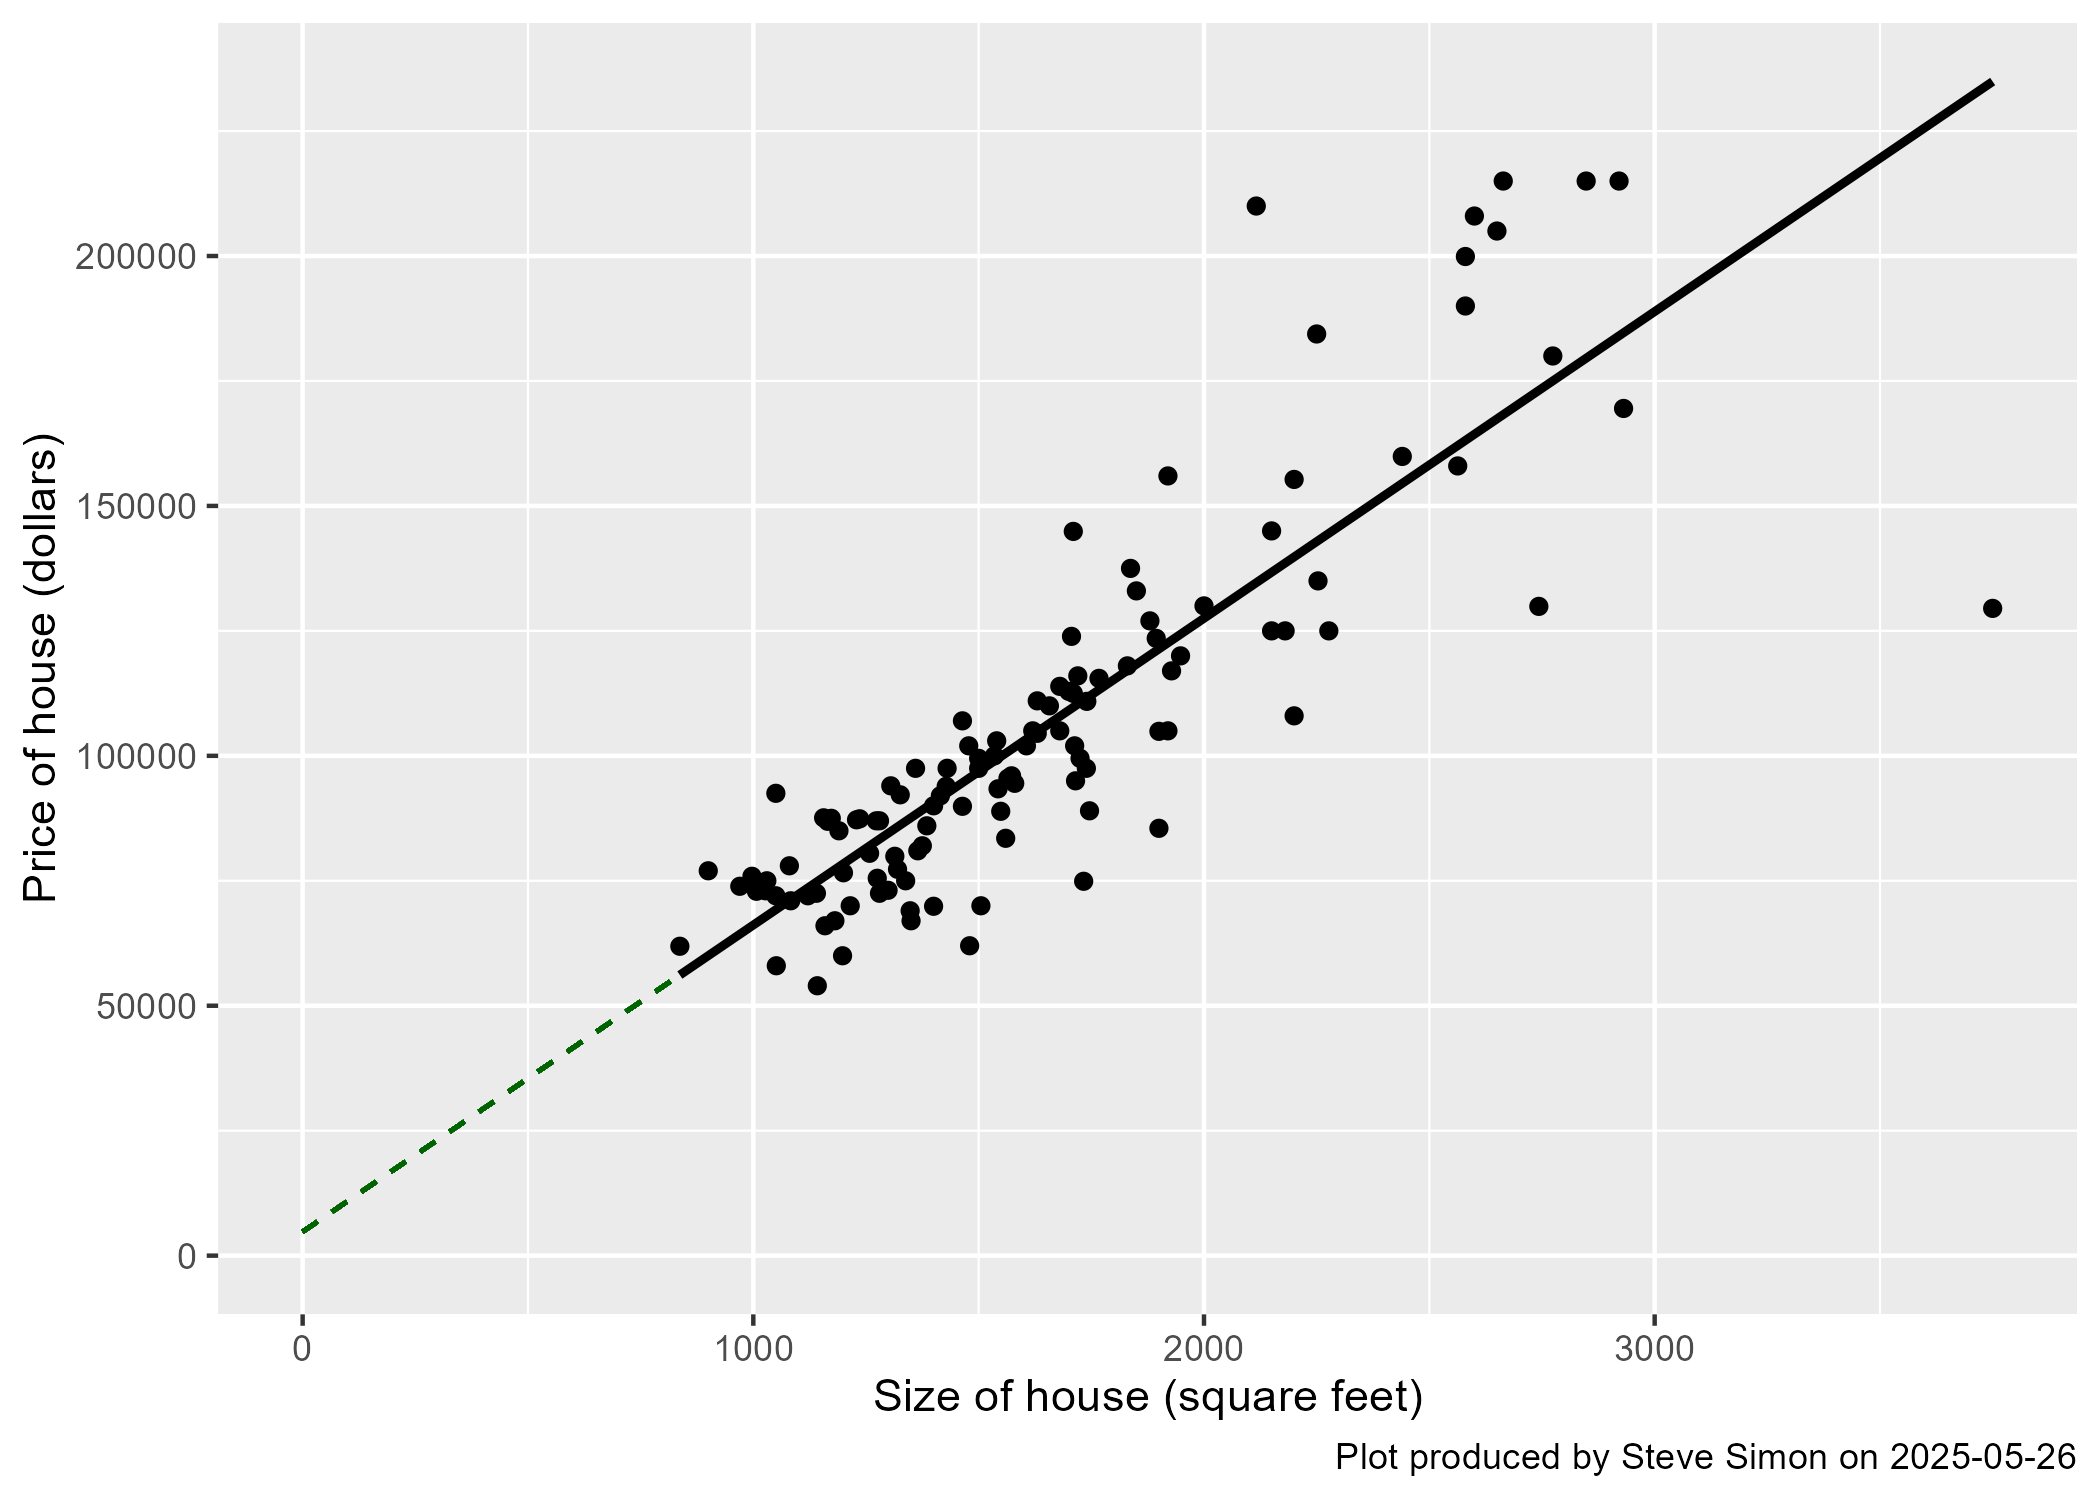
\includegraphics[keepaspectratio]{chapters/../images/figure-11-02.png}}

The intercept appears to be just a tad above zero. Call it five thousand
dollars. Now does it make sense to pay five thousand dollars for a house
of zero square feet? You might argue that the five thousand dollars
represents the estimated average price for an empty lot, perhaps.
Perhaps not. If you are a bit skeptical of this interpretation, you are
probably justified in that skepticism. It is quite a bit of an
extrapolation.

The importance of the eyeball estimates is that they greatly reduce the
fear and intimidation that you might feel when you actually run your
regression analysis. You will be looking for two friends, the slope of
around 60 and the intercept of around five thousand. When you see those
friends in your regression table, you will get some reassurance that you
are doing things properly.

Now if your regression model includes categorical variables, display
them using boxplots. You might suspect that custom built houses will be
a bit pricier, and looking at the boxplot, you'd be right!

\pandocbounded{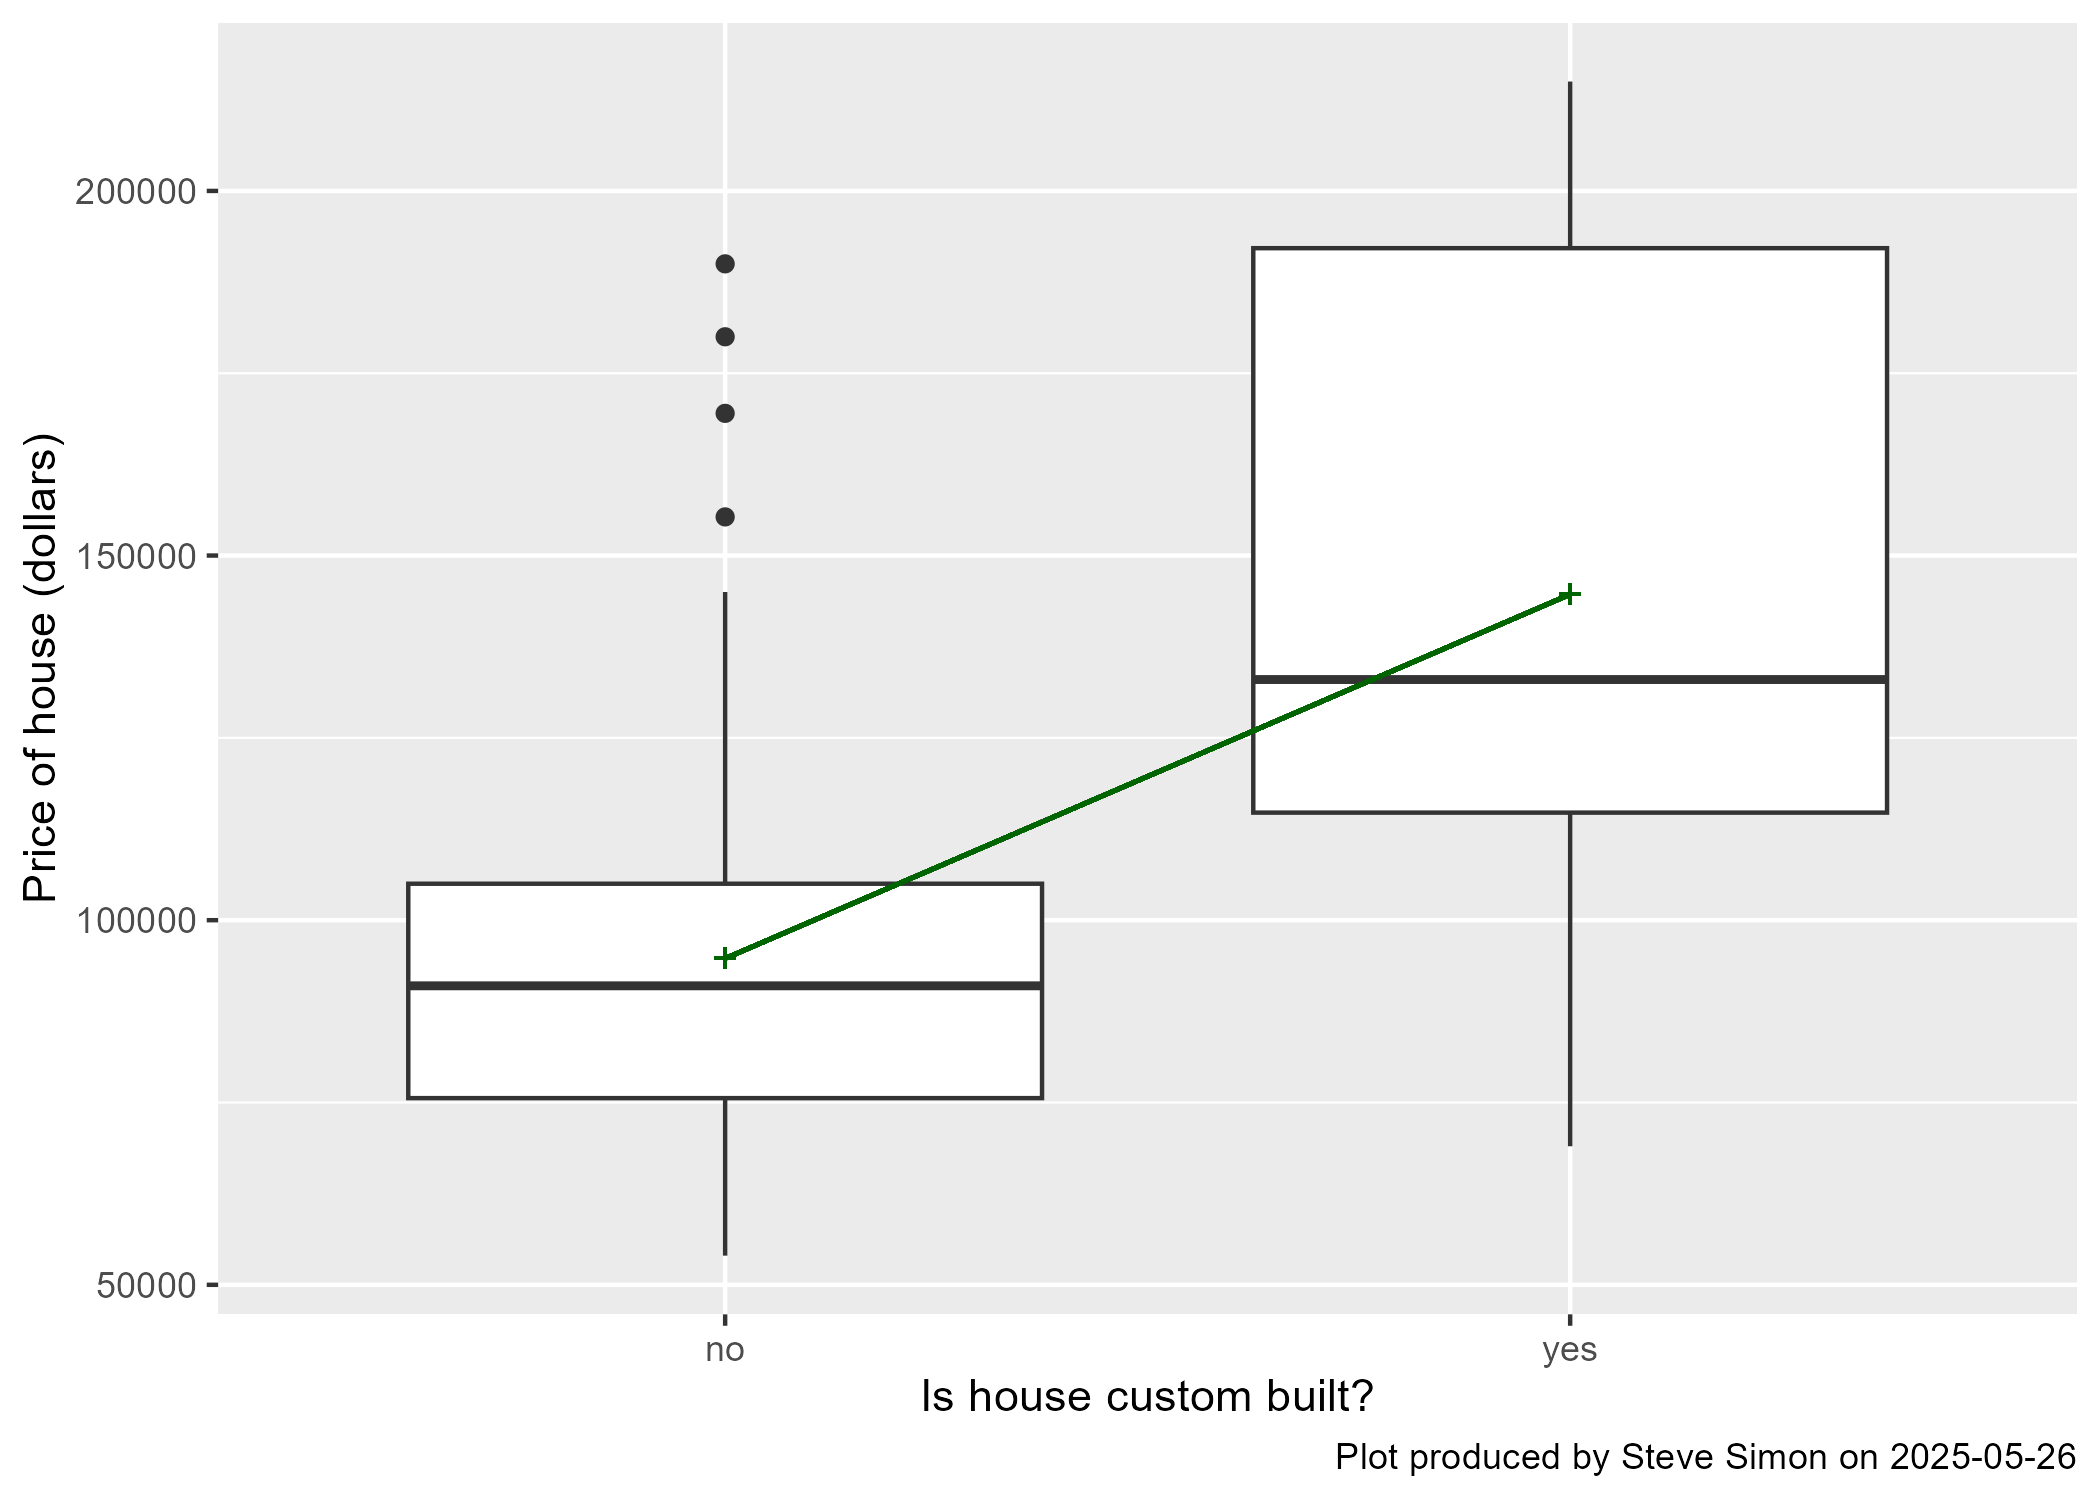
\includegraphics[keepaspectratio]{chapters/../images/figure-11-03.png}}

I added the means (small plus signs) and a line connecting them to this
boxplot. The estimated average price of a regular home appears to be
around 95 thousand dollars. The average price for a custom-built house
is around 145 thousand dollars, about 50 thousand dollars more. When you
run the regression model predicting price from the custom-built
indicator, look for two friends, a slope of 50 thousand dollars and an
intercept of 95 thousand dollars.

If you plan to look at the joint effects of size and custom-built, take
some time to evaluate how these two independent variables relate to one
another. A boxplot works well here.

\pandocbounded{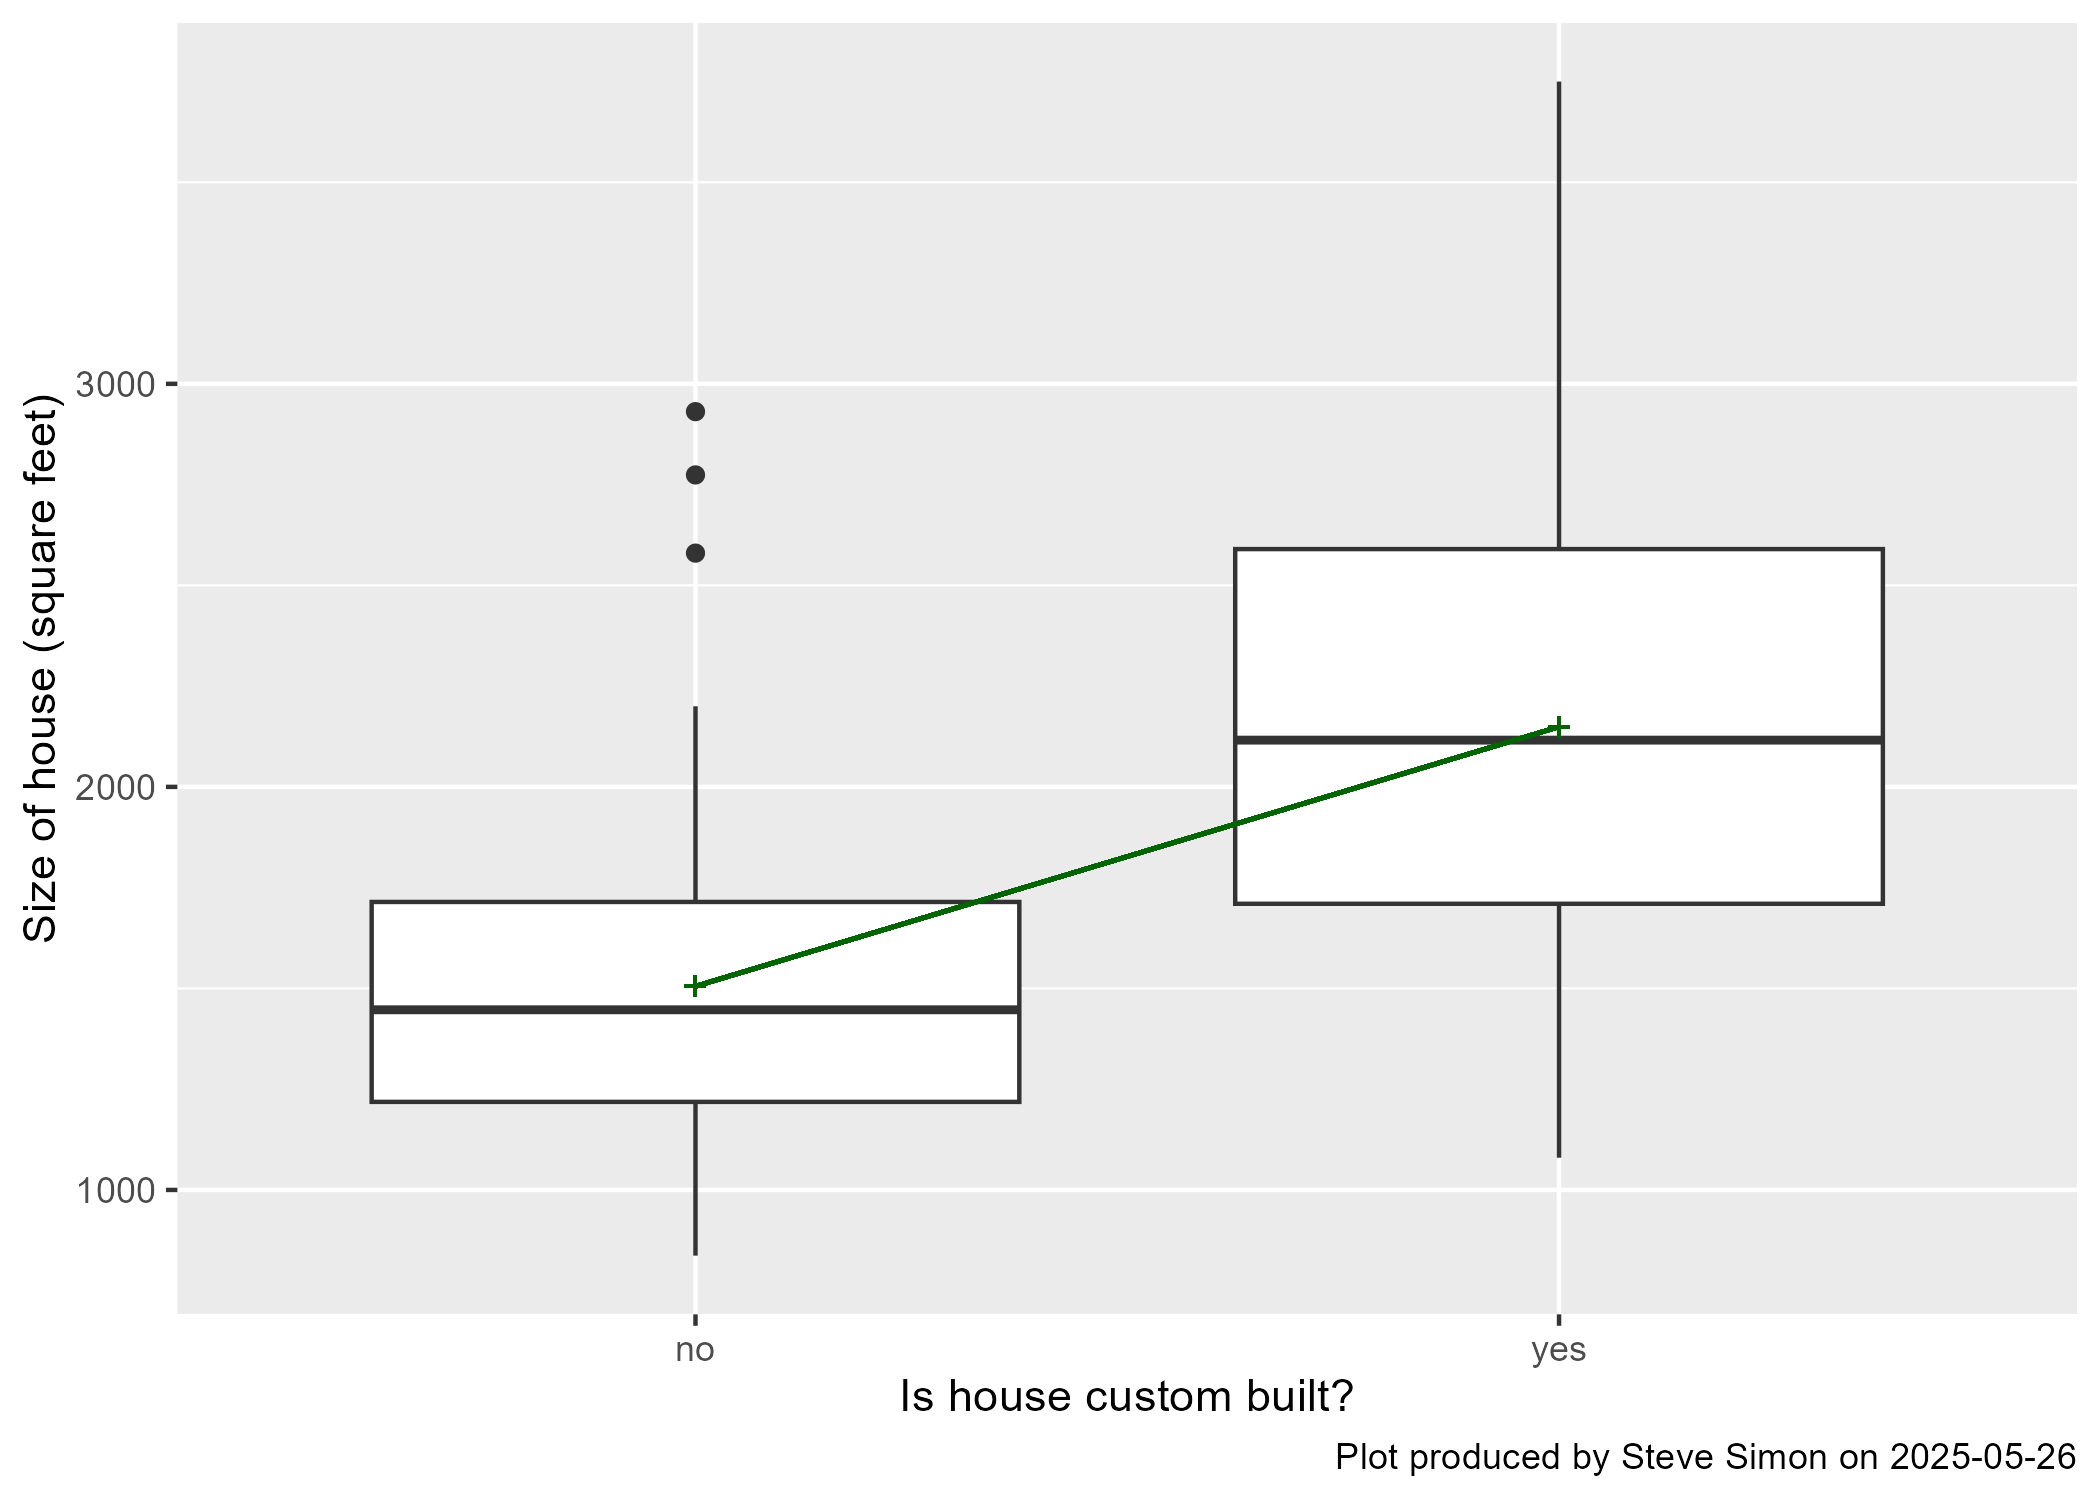
\includegraphics[keepaspectratio]{chapters/../images/figure-11-04.png}}

This box plot shows an interesting pattern that you probably were
expecting. Custom-built houses are also bigger houses. The two
independent variables are positively correlated. This is not a fatal
problem, but you should use some care when trying to disentangle the
individual effects of each variable.

Now if you have a lot of independent variables (five or more is a lot),
you may not have the time and luxury of looking at every
interrelationship among your independent variables. A correlation matrix
might still be useful. Here is the correlation matrix between the two
independent variables and the dependent variable. I am not rounding the
values here, but you should round to two significant figures in any
report that you prepare.

Table 11-1. Correlations

\begin{verbatim}
             price      sqft  i_custom
price    1.0000000 0.8447951 0.5552920
sqft     0.8447951 1.0000000 0.5201016
i_custom 0.5552920 0.5201016 1.0000000
\end{verbatim}

The correlations are all large and positive, which passes the smell
test.

\section{Step 2: Compute a simple
model}\label{step-2-compute-a-simple-model}

There are two types of models, crude models and adjusted models. A crude
model looks at how a single factor affects your outcome measure and
ignores potential covariates. An adjusted model incorporates these
potential covariates. Start with a crude model. It's simpler and it
helps you to get a quick overview of how things are panning out. Then
continue by making adjustments for important confounders.

A crude model for comparing duration of breast feeding to feeding group
would be a t-test. I prefer

however to present a general linear model because it provides a unifying
framework for diverse statistical methods like analysis of variance
analysis of covariance, multiple linear regression repeated measures
designs and t-tests. Shown below is the table of tests from the general
linear model procedure.

The general linear model uses an F test instead of the t test

but in this context these two tests are mathematically equivalent. The
p-value for comparing feeding groups is .001 which indicates a
significant difference between the two groups. The general linear model
also has a table of estimates

which is presented below.

The intercept represents the average duration of breast feeding for the
NG tube group. We see that the average duration is 20 weeks for the NG
tube group. The (FEED\_TYP=1) term is an estimate of how much the
average duration changes when we move from the NG tube group to the
bottle group. We see that the bottle group has an average duration that
is 7 weeks shorter.

Shown below is a table of means from the general linear model.

We see that the difference between the two means is roughly 7 weeks,
which confirms the results shown previously.

\section{Step 3: Compute an adjusted
model}\label{step-3-compute-an-adjusted-model}

but could some of all of this difference be due to the fact that the NG
tube group had older mothers? To answer this we need to fit an adjusted
model. Shown below is the table of tests for a general linear model that
includes mother's age in the model.

This table shows that the effect of bottle feeding is to decrease
duration of breast feeding by about six weeks

after adjusting for mother's age. Each year that a mother is older
increase the duration of breast feeding by a quarter of a week. A
previous descriptive analysis of this data revealed that the average age
for mothers in the treatment group is 29 years and the average age for
mothers in the control group is 25 years. When you see a discrepancy
like this in an important covariate

you need to assess whether the four year gap in average ages could
account for part or all of the effect of the treatment group. This
analysis shows that the four year gap only accounts for a small portion
of the difference. Since each year of age changes the duration by a
quarter week

this means that the difference between mother's ages acounts for just
one week in the 7 week difference we saw in the crude model. Shown below
is the table of means.

This table now adjusts for mother's age. The mean for the bottle fed
group is adjusted upward to what it would be if the average age of the
mothers in this group were 27 rather than 25. The mean for the NG tube
group is adjusted downward to what it would be if the average age were
27 instead of 29. Note that the adjusted mean duration is half a week
higher than the crude mean duration in the bottle group and that the
adjusted mean duration is half a week lower than the crude mean duration
for the NG tube group. This confirms that the difference between the two
feeding groups is roughly 6 weeks

after adjusting for mother's age. This is one week less than the crude
model. This is not the final model. We should examine the effect of
delivery type and account for the fact that we have some data on twins.
I hope, though

that this presentation gives you a general idea of what crude and
adjusted models are.

\section{The fly in the ointment: clustered
data}\label{the-fly-in-the-ointment-clustered-data}

Add text.

Linear regression models provide a good way to examine how various
factors influence a continuous outcome measure. There are three steps in
a typical linear regression analysis.

Fit a crude model Fit an adjusted model Analyze predicted values and
residuals These steps may not be appropriate for every linear regression
analysis, but they do serve as a general guideline. In this presentation

you will see these steps applied to data from a breast feeding study
using SPSS software. This presentation can only give the briefest
introduction to this area. When I have time

I hope to add additional web pages to provide a more thorough approach
to this topic. **Step 1

Fit a crude model\textbf{ }Step 2

Fit an adjusted model** The previous model was a crude model. We see a
seven week difference between the two groups

The p-value for feeding group is .009

which is still significant even after adjusting for the effect of
mother's age. Shown below is the table of estimates from the same
general linear model.

**Step 3

Analyze predicted values and residuals**. A regression model gives you
an equation that you can use to compute predicted values and residuals.
In the regression model with mother's age and feeding type

the equation (with a bit of rounding) is age\_stop = 13 + 0.25 * age - 6
* feed\_typ,

where feed\_typ=1 if control

0 if treatment. So

for example if you recruited a mother into the treatment group and she
was 30 years old you would predict the duration of breast feeding to be
predicted age\_stop = 13 + 0.25 * 30 - 6 * 0 = 20.5 weeks.

If you recruited a mother into the treatment group and she was 19 years
old

you would predict the duration of breast feeding to be predicted
age\_stop = 13 + 0.25 * 19 - 6 * 0 = 17.75 weeks.

If you recruited a mother into the control group and she was 37 years
old

you would predict the duration of breast feeding to be predicted
age\_stop = 13 + 0.25 * 37 - 6 * 1 = 16.25 weeks.

Now it turns out that the first three rows of your data set correspond
to the three scenarios described above. The actual values we observed
were 30 weeks

4 weeks and 12 weeks. The residual is the difference between what we
observed in the data and what the regression model would have predicted.
For the first mother in the sample

you can observe that there are 30 weeks of breast feeding, but the model
predicted much less 20.5 weeks. You can compute residual = 30 - 22.5 =
7.5.

When the residual is positive

your regression model has under-predicted the outcome. With the second
mother your regression model has over-predicted the outcome. The
observed value is 4 and the predicted value is 17.75. So you can compute
residual = 4 - 17.75 = -13.75.

This residual is negative. For the third mother

the residual is also negative. residual = 12 - 16.25 = -4.25.

Most statistical models require certain assumptions to be made about
your data. These assumptions can be examined using residuals. If your
model is good

the residuals show a random featureless scatter. If instead they show a
systematic trend or pattern then you can improve by incorporating that
trend or pattern into your model. The simplest plot is a plot of
predicted values versus residuals (shown below).

The relatively random scatter of data values provides us with confidence
in the assumptions of the linear model. There is no obvious trend or
pattern in this plot.

I also looked at the residuals versus the feeding groups and versus
mother's age. Both showed no systematic trend or pattern (graphs not
shown).

The following plot examines normality of the residuals.

The curved line indicates a non-normal distribution. Further
investigation would identify that this distribution is rectangular: it
has a sharp lower and upper bound that differs from a bell shaped curve.
The design of this study produces these limits because the age at which
the mother stops breast feeding can't be shorter than 0 weeks and it
can't be longer than the duration of the study (roughly 6 months). In
practice

this type of non-normality is not a serious problem. Summary

There are three steps in a typical linear regression model analysis.

Fit a crude model. Fit an adjusted model. Examine predicted values and
residuals. You can find an earlier version of this page on my original
website.

Excluding direct quotes from outside sources, all text is in the public
domain. Images are copyrighted unless noted

\section{Bibliography}\label{bibliography-3}

UCLA Statistical Consulting Group. Regression Analysis \textbar{} SAS
Annotated Output. Available in
\href{https://stats.oarc.ucla.edu/sas/output/regression-analysis/}{html
format}.

Steve Simon. Steps in a typical linear regression analysis. PMean blog,
1999-09-21. Available in
\href{http://new.pmean.com/steps-in-linear-regression/}{html format}.

Steve Simon. Interpreting coefficients in a linear regression model.
PMean blog, 2002-06-24. Available in
\href{http://new.pmean.com/intepreting-linear-regression-coefficients/}{html
format}

Steve Simon. Building a complex model. PMean blog, 2003-04-23. Available
in \href{http://new.pmean.com/building-complex-models/}{html format}.

Steve Simon. Joke about the dangers of extrapolation. Pmean blog,
2021-11-27. Available in
\href{http://new.pmean.com/extrapolation-joke/}{html format}.

\bookmarksetup{startatroot}

\chapter{Running a logistic regression
analysis}\label{running-a-logistic-regression-analysis}

This chapter is based on
\href{http://new.pmean.com/steps-in-linear-regression/}{Steps in a
linear regression analysis} published 2001-10-11. Also refer to
\href{http://www.pmean.com/10/Contents.html}{Tentative table of
contents}.

\section{Step 1: Examine raw
probabilities}\label{step-1-examine-raw-probabilities}

Examine raw probabilities using crosstabs

Add text.

\section{Step 2: Compute a simple
model}\label{step-2-compute-a-simple-model-1}

Add text.

\section{Step 3: Compute an adjusted
model}\label{step-3-compute-an-adjusted-model-1}

Add text.

\section{The fly in the ointment: clustered
data}\label{the-fly-in-the-ointment-clustered-data-1}

Add text.

\bookmarksetup{startatroot}

\chapter{Running a multi-factor analysis of variance
model}\label{running-a-multi-factor-analysis-of-variance-model}

This chapter is based on \href{http://www.pmean.com/posts/anova/}{Steps
in a typical ANOVA model} published 2002-10-11. Also refer to
\href{http://www.pmean.com/10/Contents.html}{Tentative table of
contents}.

\section{Step 1: Plot clustered
boxplots}\label{step-1-plot-clustered-boxplots}

Look for interactions

\section{Step 2: Fit individual
models}\label{step-2-fit-individual-models}

Add text.

\section{Step 3: Fit multi-factor
models}\label{step-3-fit-multi-factor-models}

Add text.

\section{The fly in the ointment: unbalanced
data}\label{the-fly-in-the-ointment-unbalanced-data}

Add text.

\bookmarksetup{startatroot}

\chapter{Running a survival data
analysis}\label{running-a-survival-data-analysis}

This chapter is based on
\href{http://www.new.pmean.com/steps-in-survival-analysis/}{Steps in a
typical survival data analysis} published 2002-10-11. Also refer to
\href{http://www.pmean.com/10/Contents.html}{Tentative table of
contents}.

\section{Step 1: Plot Kaplan-Meier curves for each
group}\label{step-1-plot-kaplan-meier-curves-for-each-group}

Examine raw probabilities using crosstabs

Add text.

\section{Step 2: Compute a simple surivival
model}\label{step-2-compute-a-simple-surivival-model}

Add text.

\section{Step 3: Compute an adjusted survival
model}\label{step-3-compute-an-adjusted-survival-model}

Add text.

\section{The fly in the ointment: time-varying
covariates}\label{the-fly-in-the-ointment-time-varying-covariates}

Add text.

\bookmarksetup{startatroot}

\chapter{Running a non-linear regression
analysis}\label{running-a-non-linear-regression-analysis}

This chapter is based on
\href{http://new.pmean.com/fitting-s-shaped-curves/}{S-shaped curves}
published 2004-02-12. Also refer to
\href{http://www.pmean.com/10/Contents.html}{Tentative table of
contents}.

\section{Step 1: Plot your data}\label{step-1-plot-your-data-1}

Look for interactions

\section{Step 2: Explore your
function}\label{step-2-explore-your-function}

Add text.

\section{Step 3: Fit your model}\label{step-3-fit-your-model}

Add text.

\section{The fly in the ointment: ill-conditioned
models}\label{the-fly-in-the-ointment-ill-conditioned-models}

Add text.

\bookmarksetup{startatroot}

\chapter{Running a systematic
overview}\label{running-a-systematic-overview}

This chapter is based on {[}So you're thinking about a systematic
overview{]}{[}sim\_sys{]} published 2016-06-17. Also refer to
\href{http://www.pmean.com/10/Contents.html}{Tentative table of
contents}.

\section{Step 1: Write a protocol}\label{step-1-write-a-protocol}

Look for interactions

\section{Step 2: Collect references}\label{step-2-collect-references}

Add text.

\section{Step 3: Extract information}\label{step-3-extract-information}

Add text.

\section{The fly in the ointment: extreme
heterogeneity}\label{the-fly-in-the-ointment-extreme-heterogeneity}

Add text.

{[}sim-sys{]}

\bookmarksetup{startatroot}

\chapter{Running a focus group}\label{running-a-focus-group}

This chapter is based on a blog post I wrote in 2004 and slides from a
course I have taught on Clinical Research Methodology.

\section{Step 1: Select a theoretical
framework}\label{step-1-select-a-theoretical-framework}

Look for interactions

\section{Step 2: Write probe
questions}\label{step-2-write-probe-questions}

Add text.

\section{Step 3: Revise your questions as you learn from each focus
group}\label{step-3-revise-your-questions-as-you-learn-from-each-focus-group}

Add text.

\section{The fly in the ointment:uneven
participation}\label{the-fly-in-the-ointmentuneven-participation}

Add text.

\section{Bibliography}\label{bibliography-4}

Simon SD. Focus groups and qualitative research. Pmean blog, 2004-04-13.
Available in \href{http://pmean.com/posts/focus-groups-are-great/}{html
format}

Simon SD. simon-5510-10-slides. PMean github repository. Available in
\href{https://github.com/pmean/classes/blob/master/clinical-research-methodology/10/results/simon-5510-10-slides.pdf}{pdf
format}.

\bookmarksetup{startatroot}

\chapter{Writing a literature review}\label{writing-a-literature-review}

This material is based loosely on a web page that I wrote in 2019 and a

\section{Step 1: Organize your
references}\label{step-1-organize-your-references}

Add text

\section{Step 2: Decide on an organizing
principle}\label{step-2-decide-on-an-organizing-principle}

Add text.

\section{Step 3: Build transitions}\label{step-3-build-transitions}

Add text.

\section{The fly in the ointment: too many/too few
references}\label{the-fly-in-the-ointment-too-manytoo-few-references}

Add text.

\section{Bibliography}\label{bibliography-5}

Gabriel D. How to write a literature review. Blog post 2017-08-21.
Available in
\href{https://deborahgabriel.com/2017/08/21/how-to-write-a-literature-review/}{html
format}.

Simon SD. Writing the introduction section of a research thesis or
dissertation. Pmean blog, 2019-03-29. Available in
\href{http://pmean.com/posts/introduction-section/}{html format}.

\bookmarksetup{startatroot}

\chapter{Writing a methods section}\label{writing-a-methods-section}

This chapter is based on web pages I wrote in 2011 and 2019.

When I write a methods section, I say that any moron can do this
research and then prove it by doing it myself.

That's a bad joke, and the methods section is not written for morons. It
is written for two well-educated audiences: appraisers (readers who want
to make a critical appraisal of your work) and replicators (readers who
want to replicate your work).

The appraisers want to know if your research meets acceptable standards.
For these readers you want to brag about the things you did well. At the
same time, be honest about any compromises that you had to make. Don't
ask your reader to read between the lines. If you couldn't use blinding,
say this. Trying to hide things won't work. Most critical appraisals
will assume that no news is bad news. They will infer that only did you
do something bad, but you were too naive to even recognize that it was a
bad thing.That's okay, but your failure to mention the bad news will
brand you as naive.

The replicators ant to understand exactly what you did and how you did
it because they want to do something just like you did, possibly with
some extensions and improvements. For this audience, you need more
details, but not every last detail. Remember that anyone who wants to do
something like what you did is reasonably well educated. Assume that
they can do the routine stuff, and only document things that are tricky.
Include references, if needed.

There is going to be a tension between making the appraisers happy and
making the replicators happy. One thing that will help is that you can
make some pretty strong assumptions about the two types of readers. If
one of your methods is assessing a rectal temperature, skip the details.
The replicators already know how to do this and the appraisers don't
want to know how to do this.

There's lots of guidance on how to organize your subsections inside
methods.

Richard Kallet has a nice publication in Respiratory Care.

\begin{itemize}
\tightlist
\item
  Subjects,
\item
  Ethical considerations,
\item
  Preparations,
\item
  Protocol design,
\item
  Measurements and calculations,
\item
  Data analysis
\end{itemize}

Elena Kallestinova's publication in the Yale Journal of Biology and
Medicine provides a structure through a series of questions.

\begin{itemize}
\tightlist
\item
  What materials did you use?
\item
  Who were the subjects of your study?
\item
  What was the design of your research?
\item
  What procedure did you follow?
\end{itemize}

The International Committee of Medical Journal Editors have published a
general guide to writing a paper with a fair amount of detail about what
goes in the methods section.

\begin{itemize}
\tightlist
\item
  Selection and description of participants,
\item
  Technical information,
\item
  Statistics.
\end{itemize}

Asghar Ghasemi and others have a nice publication in the International
Journal of Endocrinology and Metabolism with only two major sections
(but several subsections in each).

\begin{itemize}
\tightlist
\item
  Materials (Chemical, Experimental materials, Experimental animals,
  Human subjects),
\item
  Methods (Study design, Measurements/assessments, Statistical analyses)
\end{itemize}

Are you confused yet? Don't despair. The fact that there are so many
different standards out there means that you have a lot of latitude in
how to structure your methods section. The best advice I can offer is to
read a half dozen articles or theses and take notes about what these
writers did. Use these suggestions more to assure that you have included
all the relevant details, but don't follow any structure mindlessly.
Don't include a subsection on chemicals if your research didn't use any
chemicals.

My recommendation is to describe two things, the who and the how, and
then lay out a statistical analysis plan. One important dividing line is
that anything that you learn after you start recruiting patients belongs
in the results section. The methods section should only include what you
knew at the start of the study. One possible exception is a description
of how many patients were lost along the way. This is often done as a
flow chart, as described below.

\section{Step 1: Talk about who}\label{step-1-talk-about-who}

Exactly who is in your study? This description will allow appraisers to
answer a key Evidence-Based-Medicine question: how similar are my
patients to those in your study. A demographic profile actually belongs
as the very first table in your results section, but there are other
important details that you should document in your methods section.

Tell us where you found your patients. Did they visit your clinic or did
they respond to an advertisement? This is an important distinction.
Patients who respond to an advertisement are going to have a different
set of motives, especially if your ad includes a monetary incentive.
This can influence the generalizability of your results.

Tell us when you found your patients. A range of dates will help your
appraisers to decide if your results are stale, meaning that they were
treated during a time when things were different. Explain if the
patients were recruited prospectively or from retrospective records.

Not everyone gets in. Tell us, in detail, any inclusion and exclusion
criteria. Document any special efforts that you take to insure
representativeness. Be honest about any limitations (both here and in
your discussion section) to representativeness that might make it more
difficult to extrapolate your results to new patients.

You are going to lose patients during the process, either through
deliberate efforts on your end (your exclusion critieria), deliberate
efforts on their end (withdrawal from the study), or logistical problems
(missed apointments, broken machinery). Document these using a flow
chart. The CONSORT (Consolidated Standards of Reporting Trials) working
group has recommended format for this chart.

Most (but not all) clinical research requires review for ethical and/or
privacy concerns. Document any approvals (for example, from
Institutional Review Boards) that you obtained before starting your
research. If your protocol was published in a clinical trial registry
(like clinicaltrials.gov), provide those details as well.

\section{Step 2: Talk about how}\label{step-2-talk-about-how}

How you do your research can fall into three general categories:
materials, procedures, and measures.

If you use any exotic supplies or chemicals, describe them here. List
the company where you procured them if they are not commonly available.
By exotic, I mean not in general use, and/or hard to find. Don't
document materials if they are not exotic. Ringers solution is not
exotic.

Documentation of procedures is similar to documentation of materials.
You only need to document the non-routine procedures. This might involve
the details on running complex equipment or the steps in an extensive
laboratory method. If these procedures are described in a peer-reviewed
publication, you might want to include that reference here. In general,
a basic procedure does not need documentation, but there are exceptions.
You might take the time to document an assessment of blood pressure if
it was done on a leg rather than an arm.

Document some (but not necessarily all) of your measures Don't describe
every single measurement, just those that are important. This, I admit,
is a judgment call.

What are the important measures? Outcome measurements are important. An
outcome measurement is one that helps you assess safety or efficacy.

Independent variables are important. These are measures that you are
interested in examining how they influence the outcome.

These variables could represent a new intervention that you give to some
of your patients versus a standard of care or a placebo, There are, sad
to say, more than a few interventions that were tested and found out to
do more harm than good.

Independent variables might instead represent exposures. An exposure is
not under your control. Exposures could be helpful or could be harmful,
but they always represent variables that you, the researcher, do not
wish to control or variables that you cannot control.

Covariates are important. Covariates are variables that you are not
interested in examining directly but which you must account for in a
proper study. Often, these are variables that already have a well
established connection to the outcome and failure to account for them
would sink the credibility of your research.

No cancer study, no matter what the treatment or exposure, would fail to
ask for information about smoking. Those cigarettes don't just cause
lung cander. They cause kidney cancer, liver cancer, that funny thing
hanging in the back of your throat cancer. Failure to control for or
adjust for smoking is a fatal flaw.

Likewise, any study in neonatology has to account for gestational age
and birthweight. Babies that arrive early and arrive tiny have so many
more problems than the later, bigger babies. Again, failure to account
for these covariates would be a fatal flaw.

Intermediate measurements are sometimes important. Intermediate
measurements are variables which are possibly influenced by your
independent variables and which, in turn, might possibly influence the
outcome. Often these variables help you to understand how a treatment
worked or why it failed.

There might be other variables, such as those that you collect during
the initial interview to see if a patient qualifies for your study.
These probably do not need to be documented.

You should present information about the validity/reliability of any
variable that warrants it. Definitely include information about
validity/reliability for key outcome measures, if they are available.
This information adds credibility to your study. For other variables,
this is a judgement call. Variables that require subject assessment,
either by the treating physician or by the patients themselves, can
often benefit from an assessment of validity/reliability.

For all of these measures, be sure to mention anything special that you
did to improve the quality of those measures. you might make
measurements in a blinded fashion, take repeated measurements, or get
measurments from two or more observers. All of these can help and are
worth bragging about.

Some studies might require you to document dozens, and sometimes even
hundreds of measures. Consider using a table for some or all of these
measures.

\section{Step 3: Talk about your analysis
plan}\label{step-3-talk-about-your-analysis-plan}

Analysis. Describe how you plan to analyze your data. Most analyses
start with some simple descriptive statistics: means and standard
deviations for continuous variables and percentages for categorical
variables.

Provide your research hypothesis in this section, and state whether it
is one-sided or two-sided. One-sided hypotheses require a brief
justification, along with an assurance that the direction of the
hypothesis was selected prior to data collection. Mention the
statistical test that you plan to use. If you are running more than one
test, explain what measures you will use to control the Type I error
rate. In some settings, it may be acceptable to not make adjustments for
multiple tests, but you should state this explicitly.

You do not need to provide references for simple and commonly used
statistics, like a t-test, linear or logistic regression, or analysis of
variance. More complex procedures should include a reference. If you are
referencing a book, remember that a page or page ranges are needed.

You need to define how you will handle missing values and dropouts. If
you plan to exclude extreme values (outliers) from your data set, give
an objective rule here.

Specify what statistical software you plan to use for your analysis
(e.g., SPSS, SAS, or R) and be sure to include the version number. State
any special libraries or macros that you used within your statistical
software system. If your software is relatively uncommon, be sure to
include a reference that explains how the software works and where you
can obtain it.

You also need to justify your sample size, and this usually fits best in
the analysis section. If the goals of your research are qualitative,
then the sample size justification can also be qualitative.

\section{The fly in the ointment: when your who is a
what}\label{the-fly-in-the-ointment-when-your-who-is-a-what}

In clinical research, the unit of analysis is almost always an
individual patient. Sometimes the unit of analysis might be a caregiver
instead, but this changes very little in how you write your methods
section. A problem occurs, however, when you are studying other than a
patient or caregiver. The environment that you are a part of, where you
live and where you work, can play such an important role in your health.
How do you write a methods section when you are studying an environment,
like a home or workplace.

Certain considerations in your methods section disappear. Houses, for
example, do not need to sign an informed consent form. You need
permission from the home owners, of course, but this is not the same
thing. Measurement of weather and/or pollutants do not raise privacy
concerns.

In place of these things, consider beefing up the details on materials
and methods. Careful assessment of environments require a great deal of
rigor. These details are critical for those replicators who want to do
similar work.

Some other details still apply. A house can meet certain inclusion and
exclusion criteria. It has a variety of measures that you need to
document. The analysis will often use the same statistical tests that
you use with a study of patients.

\section{Bibliography}\label{bibliography-6}

About ClinicalTrials.gov. Available in
\href{https://clinicaltrials.gov/about-site/about-ctg}{html format}.

Ghasemi A, Bahadoran Z, Zadeh-Vakili A, Montazeri SA, Hosseinpanah F.
The Principles of Biomedical Scientific Writing: Materials and Methods.
Int J Endocrinol Metab. 2019 Jan 28;17(1):e88155. doi:
\href{https://doi.org/10.5812/ijem.88155}{10.5812/ijem.88155}.

Hopewell S, Chan AW, Collins GS, Hróbjartsson A, Moher D, Schulz KF,
Tunn R, Aggarwal R, Berkwits M, Berlin JA, Bhandari N, Butcher NJ,
Campbell MK, Chidebe RCW, Elbourne D, Farmer A, Fergusson DA, Golub RM,
Goodman SN, Hoffmann TC, Ioannidis JPA, Kahan BC, Knowles RL, Lamb SE,
Lewis S, Loder E, Offringa M, Ravaud P, Richards DP, Rockhold FW,
Schriger DL, Siegried NL, Staniszewska S, Taylor RS, Thabane L,
Torgerson D, Vohra S, White IR, Boutron I. CONSORT 2025 statement:
updated guideline for reporting randomised trials. PLoS Med. 2025;
22(4): e1004587. PMID: {[}40228477{]}{[}ref19-hoepwell-2025{]}

International Committee of Medical Journal Editors. Preparing a
Manuscript for Submission to a Medical Journal. Available in
\href{https://icmje.org/recommendations/browse/manuscript-preparation/preparing-for-submission.html}{html
format}

Kallestinova ED. How to write your first research paper. Yale J Biol
Med. 2011 Sep;84(3):181-90. PMID:
{[}21966034{]}{[}ref19-kallestinova-2011{]}

Kallet RH. How to write the methods section of a research paper.
Respiratory Care. 2004 Oct;49(10):1229-32. PMID:
\href{https://pubmed.ncbi.nlm.nih.gov/15447808/}{15447808}.

Simon SD. Writing the methods section of your grant, Pmean blog,
2011-04-26. Available in {[}html format{]}{[}ref19-simon-2011{]}.

Simon SD. Writing the methods section of a research paper, Pmean blog,
2019-04-25. Available in
\href{http://pmean.com/posts/writing-methods-section/}{html format}

\bookmarksetup{startatroot}

\chapter{Writing a results section}\label{writing-a-results-section}

\section{Step 1:}\label{step-1}

Add text.

\section{Step 2:}\label{step-2}

Add text.

\section{Step 3:}\label{step-3}

Add text.

\section{The fly in the ointment:}\label{the-fly-in-the-ointment-5}

Add text.

\section{Bibliography}\label{bibliography-7}

Bahadoran Z, Mirmiran P, Zadeh-Vakili A, Hosseinpanah F, Ghasemi A. The
Principles of Biomedical Scientific Writing: Results. Int J Endocrinol
Metab. 2019 Apr 24;17(2):e92113. doi:
{[}10.5812/ijem.92113{]}{[}ref20-bahadoran-2019{]}. PMID: 31372173;
PMCID: PMC6635678.

\bookmarksetup{startatroot}

\chapter{Writing a discussion
section}\label{writing-a-discussion-section}

This chapter is based on \textless{}\textgreater. Also refer to
\href{http://www.pmean.com/10/Contents.html}{Tentative table of
contents}.

\emph{One of the naturalists had argued that On the Origin of Species
was too theoretical, that Darwin should have just ``put his facts before
us and let them rest.'' In response, Darwin reflected that science, to
be of any service, required more than list making; it needed larger
ideas that could make sense of piles of data. Otherwise, Darwin said, a
geologist ``might as well go into a gravel-pit and count the pebbles and
describe the colours.'' Data without generalizations are useless; facts
without explanatory principles are meaningless.} Michael Shermer, Why
Darwin Matters. The Case Against Intelligent Design. (page 1).

The discussion section of a research paper is typically the last part of
the paper that you will write, because it draws on information from the
literature review, the methods section, and the results section. It is
not a rehash of any of these sections, but rather a synthesis.

Also keep in mind that most of your readers will know less about your
research area than you do. If you leave the true significance of your
research unstated out of a sense of false modesty, your readers will
likely miss your point.

If you are stuck on writing a discussion section, here are some steps
you can take to get going again.

\begin{enumerate}
\def\labelenumi{\arabic{enumi}.}
\tightlist
\item
  Compare/contrast your results to previous results.
\item
  List the strengths and limitations of your study.
\item
  Advocate changes (or support the status quo)
\item
  Suggest areas for further research.
\end{enumerate}

\section{Step 1: Compare/contrast your results to previous
results.}\label{step-1-comparecontrast-your-results-to-previous-results.}

The literature review your wrote was your chance to lay out what was
known before you started your research. Your results section was your
chance to lay out what you found in your research. In the discussion
section, you need to combine information from both sections.

Did any of your results support what was previously done? That's great.
Brag about it! We now know certain things with much greater confidence
because your work supported and strengthened information and knowledge
in your area of work.

Did any of your results contradict what was previously done? That's
great. Brag about it! Maybe your research is correct, maybe their
research is correct. Maybe both are correct.

If you think your research is correct, explain what was different about
what you did. Speculate a bit. Did your larger sample size find things
that earlier small studies could not? Did you measure things more
carefully? Did you measure things that no one else had measured before?
have larger sample size that led to

The discussion section is also the section for speculation. Not wild
unsupported speculation, of course, but reasonable extrapolations beyond
the strict bounds of your data. If your data calls into question a
proposed mechanism of action, for example, you can suggest an
alternative mechanism. If your proposed intervention did not work as
intended, you can speculate on what changes in your intervention might
have led to a different outcome.

\section{Step 2: List the strengths and limitations of your
study.}\label{step-2-list-the-strengths-and-limitations-of-your-study.}

The discussion section is your chance to answer the ``so what'' question
about your work. You need to place your work in the context of previous
research and discuss the persuasiveness of your findings. Don't be shy
here. If your research is a lot better than any previous work, tell your
readers this. Likewise, tell your readers if you've filled an important
knowledge gap or if you've produced novel insights. In other words, brag
a little bit.

I'm holding my breath when I tell you to brag. If there's a fault with
discussion sections, it is when writers grossly overstate the
significance of their research. There is no shame in conducting and
reporting a ``weak'' research study. It only becomes a sin if you
pretend that a weak study is more definitive than it deserves to be.

But you're not one of these types. The writers who overstate things
never get stuck. You're stuck because you're too tentative. Adopting a
cautious ``yes, but'' tone has filled your heart with gloom and weighed
you down. It is better to start off brashly so as to get something down
on paper. You can always tone it down later.

\section{Step 3: Advocate changes (or support the status
quo)}\label{step-3-advocate-changes-or-support-the-status-quo}

The discussion section is also your chance to be a little bit ``bossy.''
If your research supports the need for changes in clinical practice,
tell us what you think those changes should be. If it supports a change
in regulations or laws, tell us that also. Tell us the future research
directions that your current findings might suggest.

\section{Step 4: Suggest areas for further
research.}\label{step-4-suggest-areas-for-further-research.}

Your study was not the last word in this research area. Maybe not, as
you will find out in the next section. But if it is indeed not the last
word, you should explain what comes next. Write down some suggestions
about what you'd like to see done. It doesn't have to be done by you,
but it needs to be done by somebody.

This takes your research paper full circle. You started out in your
literature review with the past, talked in the present about your own
work in the results section and to some extent in this discussion
section as well. The last part of the discussion section, though, is
about the future. Don't hold back your best ideas because you want to
reserve those ideas for you and you alone.

Back in Chapter 1, I reminded you how to get your research idea. Maybe
you had one already, and maybe you found it somewhere else. Maybe you
found it, though, in the discussion section of one of the papers in your
literature review. Even if you didn't those papers in your literature
review helped shape your research. So here's your chance to pay it
forward. Let someone else benefit from the wisdom that you have
accumulated because much of that accumulated ion was from those who came
before you.

\section{The fly in the ointment: When should research
end?}\label{the-fly-in-the-ointment-when-should-research-end}

\section{Bibliography}\label{bibliography-8}

Höfler M, Venz J, Trautmann S et al.~Writing a discussion section: how
to integrate substantive and statistical expertise. BMC Med Res Methodol
18, 34 (2018). DOI:
\href{https://doi.org/10.1186/s12874-018-0490-1}{10.1186/s12874-018-0490-1}

Simon SD. How to Write a Discussion Section. The Monthly Mean
newsletter, July/August 2012. Available in
\href{http://www.pmean.com/news/201207.html\#1}{html format}

\bookmarksetup{startatroot}

\chapter{Summary}\label{summary}

In summary, this book has no content whatsoever.

\bookmarksetup{startatroot}

\chapter*{References}\label{references}
\addcontentsline{toc}{chapter}{References}

\markboth{References}{References}

\phantomsection\label{refs}
\begin{CSLReferences}{0}{1}
\end{CSLReferences}

I'm thinking that maybe it makes more sense to put a bibliography at the
end of each chapter, but I haven't decided for sure just yet.




\end{document}
